\ifx \notincludehead\undefined
    \newcommand*{\No}{\textnumero}
 
    \documentclass[russian, utf8, 12pt, pointsubsection,floatsubsection]{eskdtext}
    \usepackage[russian]{babel}

	\ifx\pdfoutput\undefined  
		\def\pdfoutput{0}
	\fi

	\ifnum\pdfoutput=0 
		\sloppy
		%	\usepackage[dvips]{graphicx}       % загрузка графики под dvi  
		\textheight=250mm                  % для DVI высота печатного текста
		\textwidth=165mm                   % ширина печатного текста
	\else
		%	\usepackage[pdftex]{graphicx}      % загрузка графики под pdf
		\usepackage{cmap}                  % чтоб работал поиск по PDF 
		% гиперссылки в PDF
		\usepackage[unicode, pdftex, colorlinks, linkcolor=blue]{hyperref} 
		\pdfcompresslevel=9                % сжимаем PDF 
		%	\textheight=240mm                  % для PDF высота печатного текста
		%	\textwidth=165mm                   % ширина печатного текста
	\fi 

	\usepackage{eskdchngsheet}
	\usepackage[T2A]{fontenc}
	%\usepackage[cp1251]{inputenc}
	\usepackage{amstext}
	\usepackage{amsmath}
	\usepackage{listings}
	\usepackage{rotating}
	\usepackage{pmasc}
    % пакет placeins позволяет вставлять плавающие объекты (рисунки) в том месте, 
    % где это необходимо. Для вывода рисунка после него встаить команду \FloatBarrier
	\usepackage{placeins}    
    
	\usepackage{array}
	\usepackage{longtable}   % подключение длинных таблиц
	\usepackage{indentfirst} % идентификация первых абзацев после секционирования
	\usepackage{fancyhdr}    % расширенный формат страниц
	\usepackage{ulem}        % подчеркивания текста \uline\uuline\uwave\sout \xout
	%\voffset=-25mm   % -25         % сдвиг страницы вверх
	%\hoffset=-15mm   % -10         % сдвиг страницы влево
    \usepackage{graphicx}
    \usepackage{floatflt} % для рисунков
	\usepackage{wrapfig}  % для рисунков
    \usepackage{todonotes} % тудушки
	\usepackage{xspace}    % убрать лишние пробелы
	\usepackage{comment}   % комментировать блоками
    %\usepackage[usenames]{color}
    %\usepackage{colortbl}

	\sloppy                             % подавление дополнительных переносов
	\righthyphenmin=2                   % можно переносить
	
	\ESKDclassCode{ТП}
	\ESKDtitle{Программная система планирования производства ПС ПП «Opti-Paper»}

	\usepackage{lscape}

	% для Первой спецификации
	\ESKDdocName{Описание бизнес-процессов}
	\ESKDsignature{\ESKDNUM}
	\ESKDcolumnII{\ESKDNUM}
	\ESKDcolumnI{Программная документация. БП. Ред.1}

	\ESKDgroup{ООО <<Опти-Софт>>}
	\ESKDauthor{Косицын Д.П.}
	\ESKDtitleAgreedBy{Директор ООО <<Опти-Софт>>}{Шабаев А.И.}
	\ESKDtitleDesignedBy{Зам. директора <<Опти-Софт>>}{Косицын Д.П.}
    \ESKDtitleDesignedBy{Консультант}{Жернаков Р.В.}	
    \ESKDtitleDesignedBy{Начальник отдела разработки}{Сошкин Р.В.}


	\ESKDtitleApprovedBy{Генеральный директор \FIRMA}{\DIRECTOR}
	%\ESKDtitleApprovedBy{\rule{72pt}{1pt}}{\rule{72pt}{1pt}}
	\ESKDtitleAgreedBy{Директор по производству}{ФИО}
	\ESKDtitleAgreedBy{Коммерческий директор}{ФИО}

	%\ESKDtitleAgreedBy{\rule{72pt}{1pt}}{\rule{72pt}{1pt}}

	\ESKDdate{2024/11/20}
    \frenchspacing
    %	\newcommand*{\No}{\textnumero}
	% для нумерации в длинных enumerate: a, b,...y, z, aa,ab,..
	%\usepackage{alphalph}  
	%\renewcommand{\theenumi}{\alphalph{\value{enumi}}}
\fi

\def \notincludehead{}
%\newcommand*{\No}{\textnumero}

%  Текущая версия 
\newcommand{\VERSION}{1.0} 


\newcommand{\FIRMA}{АО «АВА плюс два»}
\newcommand{\firma}{АО «АВА плюс два»}
\newcommand{\CURADDRESS}{644044, Российская Федерация, город Омск, улица Электрификаторов, 5}
\newcommand{\ADDRESS}{644044, Российская Федерация, город Омск, улица Электрификаторов, 5}
\newcommand{\ESKDNUM}{65698922.425120.050.П2.\VERSION}
\newcommand{\DIRECTOR}{Аноков И.В.}
\newcommand{\curobject}{}
\newcommand{\agreement}{№ОС.К.32-24 от 09.07.2024г.}


\begin{document}

	% титульный лист 
 	\maketitle

	% содержание ЕСКД
% 		\begin{center}
		\large \textbf{СОДЕРЖАНИЕ} \normalsize
	\end{center}
	\begin{longtable}{|p{10mm}|p{10mm}|p{30mm}|p{60mm}|p{10mm}|p{25mm}|} 
	\hline

	\rotatebox{90}{\textbf{Номер строки}} &
	\rotatebox{90}{\textbf{Формат}} &
	\textbf{Обозначение} & \textbf{Наименование} & 
	\rotatebox{90}{\textbf{Кол-во листов}} & 
	\textbf{Примечание}\\
	\hline
	
	1 & A4 & & Оглавление &  & \\
	\hline
	2 & A4 & & Общие положения &  & \\
	\hline
	3 & A4 & & Назначение и цели создания системы &  & \\
	 \hline
	4 & A4 & & Характеристика объекта автоматизации &  & \\
	\hline
	5 & A4 & & Описание требований к системе &  & \\
	\hline
%	 4 & A4 & & Состав и содержание работ &  & \\
%	\hline
%	5 & A4 & & Порядок контроля и приемки работ &  & \\
%	\hline
%	 6 & A4 & & Требования к документированию &  & \\
%	\hline
%	 7 & A4 & & Приложения &  & \\
%	\hline
	\end{longtable}
%  	\newpage

	% оглавление 
	\scriptsize
	\setcounter{tocdepth}{4}
	\tableofcontents
	\normalsize
	\newpage

 		\begin{center}
		\large \textbf{СОСТАВИЛИ} \normalsize
	\end{center}
% Table generated by Excel2LaTeX from sheet 'Лист1'
\begin{longtable}{|p{40mm}|p{50mm}|p{28mm}|p{16mm}|p{16mm}|}
\hline
\parbox[c][5mm]{24mm}{\raggedrightОрганизация} & \parbox[c]{49mm}{\raggedrightДолжность исполнителя} & \parbox[c]{28mm}{\raggedrightФамилия И.О.} & \parbox[c]{16mm}{\raggedrightПодпись} & \parbox[c]{16mm}{\raggedrightДата} \\
\hline
\parbox[c][15mm]{40mm}{ООО «Опти-Софт»} & Зам директора & Косицын Д.П. &            &            \\
\hline
\parbox[c][15mm]{40mm}{ООО «Опти-Софт»} & Начальник отдела разработки & Сошкин Р.В. &            &            \\
\hline
\parbox[c][15mm]{40mm}{ООО «Опти-Софт»} & Консультант & Жернаков Р.В.&            &            \\
\hline
% \caption{}\label{}
\end{longtable}  


	\begin{center}
		\large \textbf{СОГЛАСОВАНО} \normalsize
	\end{center}
% Table generated by Excel2LaTeX from sheet 'Лист1'
\begin{longtable}{|p{40mm}|p{50mm}|p{28mm}|p{16mm}|p{16mm}|}
\hline
\parbox[c][5mm]{40mm}{\raggedrightОрганизация} & \parbox[c]{49mm}{\raggedrightДолжность исполнителя} & \parbox[c]{28mm}{\raggedrightФамилия И.О.} & \parbox[c]{16mm}{\raggedrightПодпись} & \parbox[c]{16mm}{\raggedrightДата} \\
\hline
\parbox[c][20mm]{40mm}{\firma} &   &   &            &            \\
\hline
\parbox[c][20mm]{40mm}{\firma} &   &   &            &            \\
\hline
\parbox[c][20mm]{40mm}{\firma} &   &   &            &            \\
\hline
\parbox[c][20mm]{40mm}{\firma} &   &   &            &            \\
\hline
\parbox[c][20mm]{40mm}{\firma} &   &   &            &            \\
\hline
% \caption{}\label{}
\end{longtable} 


 	
 	\newpage


\section*{История изменений}
\noindent

% Table generated by Excel2LaTeX from sheet 'Лист1'
\scriptsize
\begin{longtable}{|p{40mm}|p{20mm}|p{20mm}|p{60mm}|}
\hline
{\bf \parbox[c][5mm]{40mm}{\centering Причина}} & {\bf \parbox[c]{19mm}{\centering Дата}} & {\bf \parbox[c]{16mm}{\centering Версия}} & {\bf \parbox[c]{25mm}{\centering Автор}} \\
\hline
\parbox[c][9mm]{40mm}{Первая редакция} & \parbox{19mm}{26.11.2024} & \parbox{16mm}{1.0} & \parbox{60mm}{Жернаков Р.В.} \\
\hline
\parbox[c][9mm]{40mm}{Отправлено} & \parbox{19mm}{29.11.2024} & \parbox{16mm}{1.0} & \parbox{60mm}{Косицын Д.П.} \\
% \hline
% \parbox[c][9mm]{40mm}{Исправления п.п.2.2.1, 2.3.1, 2.4.3} & \parbox{19mm}{06.05.2024} & \parbox{16mm}{1.1} & \parbox{25mm}{Жернаков Р.В.} \\
% \hline
% \parbox[c][9mm]{40mm}{Исправления п.4.4.} & \parbox{19mm}{16.10.2023} & \parbox{16mm}{1.3} & \parbox{25mm}{Жернаков Р.В.} \\
% \hline
% \parbox[c][9mm]{40mm}{Выслано} & \parbox{19mm}{25.10.2023} & \parbox{16mm}{\VERTION} & \parbox{25mm}{Жернаков Р.В.} \\
%\hline
%\parbox[c][5mm]{40mm}{} & \parbox{19mm}{} & \parbox{16mm}{} & \parbox{25mm}{} \\
\hline
&&&\\
\hline
&&&\\
\hline
&&&\\
\hline
\end{longtable}  
\normalsize 	
 	
 	\newpage
 	
 	
 \section*{Словарь терминов и сокращений}
\noindent

\begin{tabular}{l l}
% {\bf ОКК}  & --- Отдел контроля качества.\\
% {\bf ППО}  & --- Планово-производственный отдел.\\
{\bf г/к}, {\bf ГК}  & --- Гофрокартон.\\
{\bf ГП}  & --- Готовая продукция.\\
{\bf ПФ}  & --- Полуфабрикат (заготовка).\\
% {\bf ГОГП}  & --- группа по отпуску готовой продукции.\\
{\bf ЛГК}, {\bf ГА}, {\bf Г/А}  & --- Гофроагрегат.\\
% {\bf ДП}  & --- Департамент продаж.\\
{\bf ЛП}, {\bf ПЛ}  & --- Линия переработки, перерабатывающая линия.\\
{\bf ТК}  & --- Технологическая карта.\\
	
\end{tabular}






\newcommand*{\IsScancode}{1}  % Если {1}, то соберётся файл с применением ШК
\newcommand*{\IsOKP}{0}  % Если {1}, нужно ОКП?




\newpage



% Основные роли

\newcommand{\gofro}{\blue{@ГТ}\xspace}
\newcommand{\erp}{\blue{@1С:УПП}\xspace}
\newcommand{\buh}{\blue{@1C:Бухгалтерия}\xspace}
\newcommand{\syncro}{\blue{@SYNCRO}\xspace}
\newcommand{\newkuani}{\blue{@Newkuany}\xspace}


\newcommand{\manager}{\green{!МенеджерПоПродажам}\xspace}
\newcommand{\tehnolog}{\green{!Технолог}\xspace}
\newcommand{\preproductionspecialist}{\green{!Специалист по подготовке производства}\xspace}
\newcommand{\designer}{\green{!Дизайнер}\xspace}
\newcommand{\planner}{\green{!Планировщик}\xspace}
% \newcommand{\montaznik}{\green{!Монтажник}\xspace}
\newcommand{\operator}{\green{!МашинистЛинии}\xspace}
\newcommand{\linkoperator}{\green{!ОператорРаската }}
% \newcommand{\supplier}{\green{!МенеджерПоСнабжению}\xspace}
\newcommand{\purchase}{\green{!СпециалистПоЗакупкам}\xspace}
\newcommand{\logistician}{\green{!МенеджерПоЛогистике}\xspace}
\newcommand{\processengineer}{\green{!ДиректорПоПроизводству}\xspace}
\newcommand{\auditor}{\green{!Бухгалтер}\xspace}
\newcommand{\gaoperator}{\green{!МашинистГА}\xspace}
\newcommand{\kladovshik}{\green{!Кладовщик}\xspace}
\newcommand{\master}{\green{!МастерСмены}\xspace}
\newcommand{\driver}{\green{!ВодительПогрузчика}\xspace}
\newcommand{\director}{\green{!Директор}\xspace}
\newcommand{\laborant}{\green{!КонтролерПоКачеству}\xspace}
\newcommand{\okk}{\green{!ОКК}\xspace}



\newcommand{\myobject}[1]{\blue{\##1}} % для обозначения документов и справочников
\newcommand{\myform}[1]{\blue{\$#1}} % для обозначения форм и кнопок



	% документ
% 	\section{Общие положения}
  	\section{Введение}

\subsection{Общие сведения}

В настоящем документе представлены результаты модернизации бизнес-процессов предприятия \FIRMA, связанные с внедрением ПС ПП «Гофротара», полученные на основе анализа, выполненного в рамках Договора \agreement. 


\newpage
\subsection{Роли}

\textbf{Роль (Бизнес-роль)} – совокупность задач, обязанностей и полномочий, связанных с конкретным участником бизнес-процесса, который несет ответственность за определенный набор функций, связанных между собой, и наделен определенным уровнем полномочий, позволяющим реализовать поставленные задачи.

Бизнес-роль присваивают сотруднику в зависимости или вне зависимости от занимаемой им должности.  

Бизнес-роли в бизнес-процессах разделяют на 2 типа: верхнего уровня и нижнего уровня.

\begin{itemize}
\item{\textbf{Роли нижнего уровня} – решают задачи, неся ответственность только за  выполнение своих функций.}\
\item{\textbf{Роли верхнего уровня} – решают задачи, неся ответственность за выполнение функций, назначенных ролям нижнего уровня.} \
\end{itemize}

При внедрении в компании процессно-ориентированного управления создают ролевую концепцию управления бизнес-процессами. Для этого в локальном нормативном акте описывают бизнес-роли и формулируют к ним основные требования, указывая сферу полномочий, ответственности, взаимосвязь с должностями, которые присутствуют в штатном расписании. 

Бизнес-роли должны иметь отношение и к самому процессу и к управлению процессами. 

Согласно ролевой концепции управления бизнес-процессами, участники исполняют определенные функции в рамках конкретного бизнес-процесса.

Бизнес-роли, предлагаемые в рамках модернизации бизнес-процессов предприятия, представлены в таблице \ref{bp:roles}.


\newpage

\begin{longtable}{|p{69mm}|p{100mm}|}
\hline
{\bf \parbox[c][5mm]{69mm}{\centering Наименование}} & {\bf \parbox[c]{100mm}{\centering Описание}} \\
\hline
{{\bf \parbox[c][15mm]{69mm}{\operator }}} & 
{\it Группа пользователей: ПодсистемаВыработка. Машинист линии переработки } \\
\hline
{\it {\bf \parbox[c][10mm]{69mm}{\gaoperator }}} & {\it Группа пользователей: ПодсистемаВыработка. Машинист гофроагрегата} \\
\hline
{\it {\bf \parbox[c][10mm]{69mm}{\kladovshik }}} & {\it Группа пользователей: ПодсистемаСклады. Кладовщик склада сырья и готовой продукции} \\
\hline
{\it {\bf \parbox[c][10mm]{69mm}{\manager }}} & {\it Группа пользователей: ПодсистемаПродажи, ПодсистемаТК. Менеджер отдела маркетинга и продаж, ассистент отдела маркетинга и продаж, ассистент менеджера по продажам} \\
\hline
{\it {\bf \parbox[c][10mm]{69mm}{\planner }}} & {\it Группа пользователей: ПодсистемаПланирование. Специалист по планированию производства } \\
\hline
{\it {\bf \parbox[c][15mm]{69mm}{\tehnolog }}} & {\it  Группа пользователей: ПодсистемаТК. Технолог, дизайнер, конструктор} \\
 \hline
{\it {\bf \parbox[c][15mm]{69mm}{\preproductionspecialist }}} & {\it  Группа пользователей: ПодсистемаТК. Специалист по подготовке производства} \\
%\hline
%{\it {\bf \parbox[c][10mm]{69mm}{\montaznik }}} & {\it  Группа пользователей: ПодсистемаТК. Слесарь-ремонтник монтажных форм, слесать-ремонтник печатной оснастки.} \\
% \hline
% {\it {\bf \parbox[c][10mm]{69mm}{\supplier}}} & {\it Группа пользователей: ПодсистемаСклады.
% Специалист по закупкам.}
% \\
% \hline
% {\it {\bf \parbox[c][10mm]{69mm}{\logistician}}} & {\it Группа пользователей: ПодсистемаПродажи, ПодсистемаСклады, ПодсистемаТранспорт
% Инженер отдела логистики, инженер по транспорту} \\
% & {Начальник отдела логистики} \\
\hline
{\it {\bf \parbox[c][15mm]{69mm}{\master }}} & {\it Группа пользователей: ПодсистемаВыработка. Мастер участка, который имеет право принимать выработку производственного оборудования и проверять сменные отчеты} \\
\hline
{\it {\bf \parbox[c][15mm]{69mm}{\processengineer}}} & {\it Группа пользователей: ПодсистемаВыработка. Директор по производству, роль верхнего уровня - контроль за исполнением производственных бизнес-процессов} \\
% \hline
% {\it {\bf \parbox[c][10mm]{69mm}{\prodtehnolog}}} & {\it Группа пользователей: ПодсистемаТК, ПодсистемаВыработка} \\
% Технолог производства, отвечающий за вопросы соблюдения технологии в процессе производства .}  \\
\hline
{\it {\bf \parbox[c][10mm]{69mm}{\auditor}}} & {\it Группа пользователей: Администратор. Бухгалтерия предприятия. Экономисты} \\
\hline
{\it {\bf \parbox[c][10mm]{69mm}{\director}}} & {\it  Группа пользователей: Администратор. Директор предприятия} \\
% \hline
% {\it {\bf \parbox[c][10mm]{69mm}{\laborant}}} & {\it  Группа пользователей: ПодсистемаКонтрольКачества. Лаборант отдела контроля качества.} \\
\hline
{\it {\bf \parbox[c][10mm]{69mm}{\laborant}}} & {\it  Группа пользователей: ПодсистемаКонтрольКачества. Контролер по качеству.} \\
\hline
\caption{Роли в процессах}\label{bp:roles}
\end{longtable}  
\normalsize



\subsection{ИТ-системы и сущности}

\begin{longtable}{|p{69mm}|p{100mm}|}
\hline
{\bf \parbox[c][5mm]{69mm}{\centering ИТ-системы, Сущности}} & {\bf \parbox[c]{100mm}{\centering Описание}} \\
\hline
\buh & {Информационная система  1С: Предприятие 8.3. Конфигурация «Бухгалтерия предприятия» }\\

\hline
\myobject{ПеремещениеТоваров} & Складской документ для регистрации факта перемещения товаров с одного склада на другой. \\
% \\
% \hline
% \myobject{ЗаказКлиента} & Документ ''Заказ клиента'' -- это запрос клиента на поставку ему товаров или оказание услуг в установленные сроки.  
% \\
% \myobject{РасходнаяНакладная} & Складской документ для регистрации факта отгрузки товаров со склада покупателю.
\hline
\myobject{ОтчетПроизводстваЗаСмену} & Документ предназначен для списания материалов с баланса складов и цеховых кладовых, а также работ с баланса подразделений, и их отнесения на выпущенную продукцию. Помимо материалов и работ в документе указываются выполненные работы сотрудников, которые требуется включить в себестоимость продукции. Документ является распоряжением на оформление документа выработки сотрудников.\\
% \hline
% \myobject{ПоступлениеТМЦ} & Документ ''Приобретение
% товаров и услуг'' предназначен для отражения различных операций по поступлению товаров и услуг. \\

%  \\
% \hline
% \myobject{ПередачаМатериаловВПроизводство} & Передача материалов в производство
% Документ регистрирует факты выдачи материалов со склада в производство.

\hline
\myobject{Контрагенты} & Справочник предназначен для хранения списка контрагентов. Контрагенты – это поставщики и покупатели, организации и частные лица.
\\
\hline
\myobject{Договоры} & Справочник предназначен для хранения договоров, заключенных с контрагентами.
\\
\hline
\myobject{Номенклатура} & Справочник предназначен для хранения информации о товарах, комплектах, наборах, готовой продукции, возвратной таре, полуфабрикатах, материалах, услугах, оборудовании.
\\
\hline
\myobject{Организация} & Справочник предназначен для хранения списка юридических лиц, входящих в состав предприятия (группы), а также хранения постоянных сведений о них. В этом же справочнике хранятся и сведения об индивидуальных предпринимателях, учет по которым ведется в программе.\\
\hline
\caption{Система \buh}\label{bp:system1}
\end{longtable}  
\normalsize




\begin{longtable}{|p{69mm}|p{100mm}|}
\hline
{\bf \parbox[c][5mm]{69mm}{\centering ИТ-системы, Сущности}} & {\bf \parbox[c]{100mm}{\centering Описание}} \\
\hline
\erp & {Информационная система 1С: Предприятие 8.3. Конфигурация «Управление производственными предприятием»}\\


\hline
\myobject{Заказ покупателя} & Документ «Заказ покупателя» (Заказ покупателя) предназначен для оформления предварительной договорённости с покупателем о намерении приобрести готовую продукцию под свои требования.
\\
\hline
\myobject{Заказ} & Документ «Заказ» (Заказ производства) предназначен для оформления требования для производства заданной продукции в указанном объеме к определенному сроку.
\\
\hline
\myobject{ПеремещениеТоваров} & Складской документ для регистрации факта перемещения товаров с одного склада на другой. \\
% \\
% \hline
% \myobject{ЗаказКлиента} & Документ ''Заказ клиента'' -- это запрос клиента на поставку ему товаров или оказание услуг в установленные сроки.  
% \\
% \myobject{РасходнаяНакладная} & Складской документ для регистрации факта отгрузки товаров со склада покупателю.
\hline
\myobject{ОтчетПроизводстваЗаСмену} & Документ предназначен для списания материалов с баланса складов и цеховых кладовых, а также работ с баланса подразделений, и их отнесения на выпущенную продукцию. Помимо материалов и работ в документе указываются выполненные работы сотрудников, которые требуется включить в себестоимость продукции. Документ является распоряжением на оформление документа выработки сотрудников.\\
\hline
\myobject{ПоступлениеТМЦ} & Документ ''Приобретение
товаров и услуг'' предназначен для отражения различных операций по поступлению товаров и услуг. \\
\hline
\myobject{РаспоряжениеНаОтгрузку} & Документ, предназначенный для выдачи распоряжения на отгрузку готовой продукции от менеджера, логисту и складским службам.
%  \\
% \hline
% \myobject{ПередачаМатериаловВПроизводство} & Передача материалов в производство
% Документ регистрирует факты выдачи материалов со склада в производство.
\\
\hline
\myobject{Контрагенты} & Справочник предназначен для хранения списка контрагентов. Контрагенты – это поставщики и покупатели, организации и частные лица.
\\
\hline
\myobject{Договоры} & Справочник предназначен для хранения договоров, заключенных с контрагентами.
\\
\hline
\myobject{Номенклатура} & Справочник предназначен для хранения информации о товарах, комплектах, наборах, готовой продукции, возвратной таре, полуфабрикатах, материалах, услугах, оборудовании.
\\
\hline
\myobject{Организация} & Справочник предназначен для хранения списка юридических лиц, входящих в состав предприятия (группы), а также хранения постоянных сведений о них. В этом же справочнике хранятся и сведения об индивидуальных предпринимателях, учет по которым ведется в программе.
\\
\hline
\myobject{Технологическая карта}  & Документ предназначен для хранения требований по изготовлению продукции. Содержит информацию по характеристике номенклатуры.
\\
\hline
\caption{Система \erp}\label{bp:system2}
\end{longtable}  
\normalsize





\begin{longtable}{|p{69mm}|p{100mm}|}
\hline
{\bf \parbox[c][5mm]{69mm}{\centering ИТ-системы, Сущности}} & {\bf \parbox[c]{100mm}{\centering Сущности}} \\
\hline
\gofro & Программная система планирования производства Гофротара, Opti-Corrugated\\
 \\
 \hline
\myobject{Контрагенты}  & Справочник предназначен для хранения списка контрагентов. Контрагенты – это поставщики и покупатели, организации и частные лица.
 \\
\hline
\myobject{Номенклатура} & Справочник предназначен для хранения информации о товарах, комплектах, наборах, готовой продукции, возвратной таре, полуфабрикатах, материалах, услугах, оборудовании.
\\
\hline
\myobject{ТехнологическаяКарта} & Справочник «Технологические карты» содержит информацию о технологических картах на изготовление готовой продукции. 
\\
\hline
\myobject{Заявка} & Документ «Заявка» (Заказ покупателя) предназначен для оформления предварительной договорённости с покупателем о намерении приобрести готовую продукцию под свои требования.
\\
\hline
\myobject{Заказ} & Документ «Заказ» (Заказ производства) предназначен для оформления требования для производства заданной продукции в указанном объеме к определенному сроку.
% \\
% \myobject{РаспоряжениеНаОтгрузку} & документ, предназначенный для выдачи распоряжения на отгрузку готовой продукции от менеджера складским службам
% \\
% \myobject{ОприходованиеТМЦ} & складской документ для регистрации факта поступления готовой продукции на склад.
% \\
% \myobject{ПоступлениеТМЦ} & Документ «Поступление ТМЦ» предназначен для отображения движения товарно-материальных ценностей в производстве и регистрации факта поступления материальных запасов, участвующих в производственном цикле.
% \\
% \myobject{ПеремещениеТМЦ} & Документ «Перемещение ТМЦ» предназначен для оформления операции перемещения материалов, товаров, продукции, полуфабрикатов между складами.
% \\
% \myobject{РеализацияТМЦ} & документ «Реализация ТМЦ» предназначен для отображения движения товарно-материальных ценностей в производстве и регистрации факта реализации готовой продукции заказчикам.
% \\
% \myobject{ПриемкаПолуфабрикатов} &документ «Приемка полуфабрикатов» предназначен для позаказного учета объема полуфабрикатов, который не требуется выпускать на гофроагрегате (например при использовании покупного картона).
% \\
% \myobject{СписаниеТМЦ} & складской документ для регистрации факта списания ТМЦ со склада.
\\
\hline
\myobject{ВыработкаПоПереработке}  & Производственный документ, рабочее место машиниста линии переработки. Рабочее место служит для получения плана работы линии переработки, формирования необходимых печатных форм и регистрации факта выработки готовой продукции и полуфабрикатов.
\\
\hline
\myobject{ВыработкаГофроагрегата} & Производственный документ, рабочее место машиниста гофроагрегата. Рабочее место служит для получения плана работы гофроагрегата (раскроев гофрополотна), формирования необходимых печатных форм и регистрации факта выработки полуфабрикатов (заготовок) и готовой продукции (гофролистов).
\\
\hline
\myobject{ЗаявкаНаИзготовлениеШтанц\-Формы} & Документ «Заявка на изготовление штанц-формы» служит основанием для создания или модификации оснастки (штанц-формы). В документе содержится подробная информация о штанц-форме. Документ доступен в том случае, если в настройках системы не установлена галочка в поле «Использовать упрощенный ввод оснастки».
\\
\hline
\myobject{ЗаявкаНаИзготовлениеФлексо\-Формы} & Документ «Заявка на изготовление ФПФ» служит основанием для создания или модификации оснастки (фотополимерной формы). В документе содержится подробная информация о ФПФ. Документ доступен в том случае, если в настройках системы не установлена галочка в поле <<Использовать упрощенный ввод оснастки>>.
\\
\hline
\myobject{Оснастка} & Справочник «Оснастка» содержит информацию по применяемым в ходе производства гофроупаковки фотополимерным печатным формам (ФПФ) и штанц формам. 
\\
\hline
\myobject{Организация}  & Справочник предназначен для хранения списка юридических лиц, входящих в состав предприятия (группы), а также хранения постоянных сведений о них. В этом же справочнике хранятся и сведения об индивидуальных предпринимателях, учет по которым ведется в программе. 
% \\
% \hline
% \myobject{ПретензииКонтрагентов} & Документ предназначен для регистрации поступающих от клиентов претензий по качеству продукции.
\\
\hline
\myobject{ЗаказПоставщику} & Документ «Заказ поставщику» предназначен для фиксации плана потребностей в товарно-материальных ценностях на складах и регистрации факта планирования потребности материальных запасов, участвующих в производственном цикле. Документ содержит информацию о видах ТМЦ, объемах планируемых потребностей для складов.
% \\
% \hline
% \myobject{ОбъемыРабочихЦентров} & Регистр сведений для указания ежедневных доступных мощностей по каждому рабочему центру (используется для предварительного планирования) 
\\
\hline
\myobject{СырьеДляВыработки} & Документ «Сырье для выработки» предназначен для регистрации использования сырья (рулоны бумаги и картона) на раскатах гофроагрегатов.
\\
\hline
\myobject{ВводОстатков} & Документ «ВводОстатков» предназначен для ввода остатков товаров на складах.
% \\
% \hline
% \myobject{ФормированиеПаллет} & Документ «ФормированиеПаллет» предназначен для генерации уникальных кодов паллет на готовую продукцию.
\\

\hline
\caption{Система \blue{\gofro}}\label{bp:system3}
\end{longtable}  
\normalsize





\begin{longtable}{|p{69mm}|p{100mm}|}
\hline
{\bf \parbox[c][5mm]{69mm}{\centering ИТ-системы}} & {\bf \parbox[c]{100mm}{\centering Сущности}} \\
\hline
\blue{@MSExcel} & Программа для работы с электронными таблицами, созданная корпорацией Microsoft для Microsoft Windows.\\
 \hline
\blue{@MSWord} & Программа для работы с электронными текстовыми документами, созданная корпорацией Microsoft для Microsoft Windows.\\
 \hline
%  \blue{@AutoCAD} & Программное обеспечение автоматизированного проектирования (САПР), для создания точных 2D - и 3D-чертежей изделий.\\
%  \hline
% \blue{@CorelDraw} & Графический редактор, предоставляющий собой полный набор инструментов для создания векторной графики.\\
%  \hline
\blue{@SYNCRO} & Система смены заказа на гофроагрегате Fosber\\
\hline
% \blue{@AbobeIllustrator} &	Векторный графический редактор, разработанный и распространяемый компанией Adobe Systems.\\
% \hline
% \blue{@ArtiosCAD} &	Векторный графический редактор для проектирования и разработки упаковки из картона.\\
%  \hline
\caption{Прочие системы}\label{bp:system4}
\end{longtable}  
\normalsize




 	
\newpage
\section{Описание бизнес-процессов}

В данном разделе представлено описание бизнес-процессов «как будет» после внедрения Программной системы планирования производства «Гофротара» (далее СИСТЕМА \gofro). Описаны только бизнес-процессы, которые будут затронуты в ходе использования СИСТЕМЫ \gofro. Текстовое описание бизнес-процессов для дальнейших этапов внедрения СИСТЕМЫ \gofro является первичным по отношению к иллюстрациям, приведенным в Приложениях. Иллюстрации носят информативный, вспомогательный характер и могут не отражать всех особенностей и деталей бизнес-процессов. 











\subsection{Описание бизнес-процесса «Продажа готовой продукции»}

\subsubsection{Сценарий ''Поиск потенциальных покупателей''}
\label{bp:sales_1}

\begin{enumerate}
    % \item \manager создает в системе \erp новый элемент   \myobject{Сделка}.  
    \item \manager создает в системе \erp новый элемент справочника  \myobject{Контрагенты}, заполняет карточку нового контрагента.
    \item	В системе \erp в справочнике  \myobject{Контрагенты} \manager заполняет дополнительную информацию по клиентам.
    \item	Новые записи выгружаются автоматически в систему \gofro в справочник \myobject{Контрагенты}.
% \item	После участия во встрече менеджер фиксирует в системе \gofro документ \blue{\#Встреча} с указанием контрагента, даты, места, представителей и описания протокола встречи
% \item	После проведения важного телефонного звонка \manager фиксирует в системе \gofro документ \blue{\#ТелефонныйЗвонок} с указанием даты, контрагента, абонента, предмета обсуждения.
% \item	Информация о клиенте не передается в \sbis пока для него в системе \gofro установлен статус «внутренний».
\end{enumerate}


\subsubsection{Сценарий ''Расчет стоимости изделия''}
\label{bp:sales_2}



\begin{enumerate}
\item 	\manager при получении от покупателя заявки на выпуск нового изделия (или пересчета цены по существующей позиции) должен определить требования покупателя по следующим параметрам:
\begin{itemize}
    \item  по качеству продукции на уровне марки бумаги /картона/ гофрокартона согласно принятым стандартам, а также размерам и условиям использования;
\item по объему поставок в разрезе одной заявки/месяца/года;
\item по условию вывоза продукции (самовывоз или доставка);
\item по способу упаковки и отправки товара (россыпью или на паллетах);
\item по условию оплаты (предоплата, отсрочка платежа);
\item ожидаемая клиентом цена за единицу продукции.
\end{itemize}

Также при необходимости \manager определяет требования покупателя по новому изделию:
\begin{itemize}
\item	Размеры изделия;
\item	Размеры заготовки;
\item	Марка, цвет, профиль;
\item	Файлы с дизайном печати и конструкцией ящика;
\item	Условия упаковки и отгрузки;
\item	Прочая информация по изделию.
\end{itemize}

\item	\manager на основании полученных данных выполняет расчет стоимости изделия в системе \erp. 
\item \manager создает в системе \erp документ \myobject{Заказ покупателя}, создаёт номенклатуру в системе (\myobject{Номенклатура}), выполняет расчет цены на номенклатуру,  выбирает маршрут.

\item \manager создаёт бизнес-карту в системе \erp,  указывает вариант доставки, отсрочку платежа. Система \erp рассчитывает минимальную цену продажи. \manager указывает процент рентабельности и получает цену продажи. 
% \item	\manager при выпуске более сложных изделий передает запрос на расчет по электронной почте для \tehnolog.

% Номенклатура будет в ГТ
% \item	\manager после согласования цены готового изделия создает в системе \erp при необходимости новую позицию справочника \#Номенклатура, при этом наименование новой позиции формирует из введенных параметров изделия в таблице MS Excel. 
% \item	\manager создает в системе \erp спецификацию цены на заданную дату.
% \item	\manager  в \erp печатает спецификацию.
\item	\manager после расчета цены оформляет в \blue{@MSWord} коммерческое предложение и отправляет клиенту.

\item Клиент в ответ высылает \manager  согласованное предложение с реквизитами для заключения договора. 
\item	\manager создает спецификацию и проект договора в системе \erp.

\item \manager готовит и согласует договор с заказчиком. Новый договор создается по шаблону договора.

% \item \manager готовит договор и спецификацию. В дальнейшем при создании заявок покупателя счет оформляется в системе \erp.

\item Бухгалтерия создает счет на предоплату при необходимости из системы \erp по запросу \manager.

\item Клиент подписывает договор, спецификацию. %и оплачивает счет. 
% \item После подписания клиентом договора и спецификации ассистент менеджера ОМиП передает их в бумажном виде специалистам ОМиП для
% оформления пакета документов и создания заказа в производство.
\end{enumerate}



\subsubsection{Сценарий ''Определение требований покупателя''}
\label{bp:sales_3}

\begin{enumerate}
\item	После успешного согласования договора и условий поставки \manager по продажам гофропродукции создает в системе \erp документ \myobject{Технологическая карта}.

\item \manager по продажам гофропродукции в системе \erp вводит требования по разработке нового изделия: 
(\red{УТОЧНИТЬ ПОЛЯ???}):

% \begin{enumerate}
%     \item 	Дата;
% \item 	Контрагент;
% \item 	Наименование изделия;
% \item 	Вид гофротары (тип изделия);
% \item 	Размеры изделия и  заготовки;
% \item 	Площадь;
% \item 	Марка гофрокартона (поиск по наименованию в справочнике \myobject{Марки});
% \item 	Профиль (поиск по наименованию в справочнике \myobject{Профиль}) ;
% \item 	Количество цветов;
% \item 	Паллетирование;
% \item 	Габариты пачки;
% \item 	Габариты поддона (поиск по наименованию в справочнике \myobject{Поддоны});
% \item 	Количество изделий в пачке;
% \item 	Количество пачек в ряду;
% \item 	Количество рядов;
% \item 	Количество изделий в паллете.
% \item 	Прочая информация по изделию.
% \end{enumerate}

\item \manager сохраняет документ. Система \erp автоматически создает в системе \gofro документ \myobject{ЗаявкаСпецификация}.
Обратно системе \gofro вернет ссылку на созданный документ, который будет прописан в системе \erp в документе \myobject{Технологическая карта}.

\item 	Разработка технологической карты выполняется в соответствии с процессом \textbf{“Проектирование и разработка новой продукции”} процедура \textbf{“Получение запроса на разработку новой продукции”} (подробнее в пункте \ref{bp:pm_1}).
\item \manager	после изменения \tehnolog статуса  документа \myobject{ЗаявкаСпецификация} на “Выполнен” в системе \gofro открывает форму созданного элемента \myobject{ТехнологическаяКарта}, вызывает по команде \myform{ПечатьТК} отчет «Отчет для клиента» и отправляет из системы \gofro форму в формате pdf или распечатывает, подписывает их у клиента на бумажном носителе с указанием даты подписания и фамилий лиц с последующей передачей в архив.
\manager может открыть ТК из системы \erp прямо по ссылке, указанной в документе \myobject{Технологическая карта}, при этом система \erp откроет окно ТК в системе \gofro.
\item 	При появлении замечаний от клиента \tehnolog вносит изменения в чертежи конструкции/дизайна и \manager повторно высылает  \myobject{ТехнологическаяКарта} на согласование клиенту.
\item 	После внесения изменений \tehnolog в чертежи конструкции/дизайна графики, подписанный и согласованный клиентом экземпляр чертежа конструкции/ дизайна графики может быть прикреплен в список файлов в системе \gofro в справочнике \myobject{ТехнологическаяКарта}. Служба планирования и другие службы получают последний верный вариант \myobject{ТехнологическаяКарта} в системе \gofro.
\item 	Любые изменения всех свойств элемента справочника \myobject{ТехнологическаяКарта} отслеживаются в системе \gofro с указанием пользователя и значения, которое было изменено.


\end{enumerate}




\subsubsection{Сценарий ''Заключение договора''}
\label{bp:sales_4}

\begin{enumerate}
\item \manager готовит и согласует договор и спецификацию к нему.
\item \manager создает элемент справочника \myobject{Договор} в системе \erp, заполняет карточку договора.
\item	По регламенту справочник выгружается в систему \gofro в справочник \myobject{Договор}.
% \item	\auditor сохраняет отсканированную копию подписанного договора в системе \erp в справочник  \myobject{Договор}.



\end{enumerate}


\subsubsection{Сценарий ''Передача заказа на изготовление''}
\label{bp:sales_5}


\begin{enumerate}
%\item \manager регистрирует в системе \gofro документ \myobject{Заявка} с указанием требований клиента по изготовлению продукции, сроков и объемов поставки. В помощь менеджеру система \gofro должна выводить по каждой номенклатуре текущие складские остатки готовой продукции по системе \erp (остатки загружаются в систему \gofro из системы \erp автоматически).
%\red{Нужно ли подгружать складские остатки готовой продукции из системы \erp, ГП в нашей систсеме?}
\item \manager по продажам гофропродукции создает в системе \erp документ \myobject{Заказ покупателя} с указанием требований клиента по изготовлению продукции, сроков и объемов поставки. В помощь менеджеру система \erp должна выводить по каждой номенклатуре текущие складские остатки готовой продукции, учтенной в системе \erp. Остатки ГП выводятся с учетом реализации, осуществляемой по системе \erp. 

\item При выборе номенклатуры и характеристики позиции \manager нажимает команду \myobject{ПроверитьТК}. При этом система \erp делает автоматический запрос в систему \gofro по указанной номенклатуре и характеристике и запрашивает статус технологической карты \myobject{ТК} в системе \gofro.
Наличие ТК и ее статус отображается в документе \myobject{Заказ покупателя} в системе \erp.

\item	При наличии предварительных заказов от клиентов большого объема с несколькими отгрузками в течение месяца \manager должен разбить такую заявку на несколько реальных производственных заказов на разные даты отгрузки.
% \item	\manager выполняет расчет предварительной даты производства продукции в соответствии с бизнес-процессом \textbf{“Планирование выпуска готовой продукции”}, процедура \textbf{“Предварительное планирование производства”} (подробнее в пункте \ref{bp:plan}).
\item	\manager в системе \erp проверяет по контрагенту дебиторскую задолженность.
% \item	После согласования сроков и объемов \manager в системе \erp создает счет на оплату при необходимости и выставляет его контрагенту. Затем \manager устанавливает в системе \gofro в документе \myobject{Заявка} статус «Одобрен к выпуску». 

\item	На основании одобренного документа \myobject{Заказ покупателя} в системе \erp \manager создает производственные заказы (документ \myobject{Заказ в производство}).
При этом заказ может быть создан только при готовности ТК: статус \myobject{ТК} в системе \gofro соответствует ''Активна''.
В каждом документе создается только одна строка с указанием готовой продукции.

\item \manager сохраняет созданный документ \myobject{Заказ в производство} в системе \erp, при этом документ будет автоматически выгружен в систему \gofro вместе с документом \myobject{Заказ покупателя}. 
Система \gofro вернет ссылку на созданный документ. Ссылка будет доступна в документе \myobject{Заказ в производство}. 

\item	\planner в системе \gofro забирает заказы для планирования ежедневно. В план уходят проведенные документы \myobject{Заказ} со статусом «Одобрено к выпуску».
\item	\manager в системе \gofro контролирует сроки исполнения заказов в производстве опираясь на отчеты «Портфель заказов» и «Ожидаемый выпуск» в системе \gofro.
\item	Для того чтобы заказ больше не участвовал в планировании, ему необходимо установить соответствующий статус: «Выполнен», «Отменен». Ответственный \manager в системе \gofro должен периодически пользоваться формой подбора выполненных заказов для того, чтобы установить соответствующий статус. Для тех заказов, которые выпущены не в полном объеме, но при этом отгрузка остатков не требуется, тоже необходимо устанавливать статус «Выполнен».
\item При внесении изменений в документ \myobject{Заказ} в системе \erp документ будет обновлен автоматически в системе \gofro в случае, если у документа стоит статус ''Новый''. Во всех остальных случаях изменение заказа в системе \gofro и в системе \erp запрещено. Система \erp  выдает соответствующее сообщение пользователю.
\end{enumerate}


\subsubsection{Сценарий ''Контроль дебиторской задолженности''}
\label{bp:sales_6}


\begin{enumerate}
\item	\manager выполняет контроль дебиторской задолженности в системе \erp.
% Убрали 
% \item	В документе \blue{\#Заявка} в системе \gofro{} \manager нажимает команду \blue{\$ПолучитьЗадолженность}, cистема \gofro формирует запрос в системе \erp и получает задолженность по оплате по контрагенту и договору на дату документа. Величина задолженности показана на форме документа \blue{\#Заявка} системы  \gofro.
\end{enumerate}

\subsubsection{Синхронизация с КИС}
\label{bp:sales_integration}


\begin{enumerate}
\item Выгрузка справочных данных из \gofro в \erp производится автоматически.
\begin{enumerate}
\item 	Справочник  \myobject{Контрагенты} из \erp загрузится в справочник  \myobject{Контрагенты} системы \gofro.
\item	Справочник  \myobject{Договоры} из \erp загрузится в справочник  \myobject{Договоры} системы \gofro.
\item	Справочник  \myobject{Номенклатура} по материалам из \erp загрузится в справочник  \myobject{Номенклатура} системы \gofro.
% •	Журнал #Спецификация из @СБИС загрузится в регистр  #ЦеныНоменклатуры системы @ГТ.
\end{enumerate}

% \item Выгрузка справочных данных из \gofro в \erp   производится автоматически.

% \begin{enumerate}
% \item	Справочник  \myobject{Номенклатура} по готовой продукции по номенклатурной группе ''Готовая продукция'' из \gofro загрузится в справочник  \myobject{Номенклатура} системы \erp.

% В системе \gofro есть возможность разделения номенклатур по группам. Выгрузке из системы \gofro в справочник  \myobject{Номенклатура} системы \erp могут быть переданы определенные группы.
% \end{enumerate}

\item	Документ \blue{\#Заказ покупателя} из \erp загрузится по команде пользователя  выгружается в документ \myobject{Заявка} системы \gofro. 
\item	Документ \blue{\#Заказ производства} из \erp загрузится по команде пользователя  выгружается в документ \myobject{Заказ} системы \gofro. 
% \item Данные по выработке из документов \myobject{ВыработкаГофроагрегата}, \myobject{ВыработкаПоПереработке} автоматически выгрузятся из \gofro в документы \myobject{ОтчетПроизводстваЗаСмену}{} системы \erp.
% \item	Документ \blue{\#Заявка} после проведения в системе \gofro выгружается в систему \erp в документ \blue{\#ЗаказКлиента}.



\end{enumerate} % Продажи

\subsection{Описание бизнес-процесса «Проектирование и разработка новой продукции»}

\subsubsection{Сценарий ''Получение запроса на разработку новой продукции''}
\label{bp:pm_1}

\begin{enumerate}

\item \manager получает от заказчика требования в виде чертежей, готовой ТК, образца короба, продукции или требования с указанием размеров продукции, веса вложения, прочностных характеристик и т.д.
\item \manager заполняет запрос на разработку чертежа конструкции/дизайна графики (процесс \textbf{«Продажа готовой продукции»}) в системе \erp в случае возникновения следующих потребностей со стороны клиента:
    
    \begin{enumerate}
        \item разработка нового вида продукции;
        \item внесение изменений в уже существующие чертежи конструкции/ дизайн графики;
\item изменение размера, удаление или добавление новых элементов;
\item изменение профиля;
\item при необходимости изготовления образца(ов) коробов по готовому чертежу конструкции.
    \end{enumerate}


\item	Для оформления запроса \manager вручную создает в системе \erp новую характеристику номенклатуры \myobject{Характеристика}, при этом будет создан документ \myobject{ТехнологическаяКарта}.
\item \manager сохраняет документ. Система \erp автоматически создает в системе \gofro документ \myobject{ЗаявкаСпецификация}.
Обратно системе \gofro вернет ссылку на созданный документ, который будет прописан в системе \erp в документе \myobject{Технологическая карта}.

\item Для заполнения дополнительных требований по изделию \manager по созданной ссылке переходит в системе \gofro и заполняет параметры в документе \myobject{ЗаявкаСпецификация}
\item	При наличии файлов от клиента \manager в системе \gofro прилагает их к документу \myobject{ЗаявкаСпецификация} на вкладке «Файлы».


\item \tehnolog просматривая обновления журнала документов \myobject{ЗаявкаСпецификация} обрабатывает требование на разработку ТК в системе \gofro документы со статусом ''Новый''.

% В случае разработки нестандартной продукции \tehnolog согласовывает возможность производства изделия с \processengineer.

\item \tehnolog создает предварительный чертеж (если требуется выпуск образцов) или рабочий чертеж в программе \blue{\@AutoCad}.
\item	При необходимости \tehnolog в системе \gofro должен создать элемент справочника \myobject{ТехнологическаяКарта}, в которую будут автоматически скопированы поля из документа \myobject{ЗаявкаСпецификация}, которые заполнил \manager. Правило нумерации: код техкарты – сквозная нумерация. Номер сквозной с префиксом "ГТ. . . "


\item \tehnolog 
% переводит чертежи и дизайн в формат «dxf» и 
отправляет чертеж по электронной почте изготовителю оснастки (сторонняя компания) и самостоятельно размещает заказ на изготовление штанцформы согласно процесса \textbf{«Заказ штанцевальных форм/клише и входной контроль качества»}. 

\item \tehnolog подгружает чертеж в систему \gofro в \myobject{ТехнологическаяКарта}.
%\item	\manager заказывает разработку дизайна штанцформы у сторонней компании согласно процесса \textbf{«Заказ штанцевальных форм/клише и входной контроль качества»}. 

\item \tehnolog «привязывает» полученный файл с разверткой штанцформы в соответствующих полях справочника \myobject{ТехнологическаяКарта}.

\item \manager при необходимости в системе \gofro размещает заказ на изготовление печатной формы согласно процесса \textbf{«Заказ штанцевальных форм/клише и входной контроль качества»}. 


% \item \tehnolog разрабатывает дизайн на основании требований \blue{\#ЗаявкаСпецификация} в системе \blue{\@CorelDraw}.
\item \tehnolog подгружает макет печати в систему \gofro в \myobject{ТехнологическаяКарта}.

\item	\manager заказывает дизайн печатной формы у компании поставщика согласно процесса \textbf{«Заказ штанцевальных форм/клише и входной контроль качества»} (подробнее в пункте \ref{bp:toolrequest}). Полученный макет \manager пересылает \tehnolog по почте или добавлением в документ \myobject{ЗаявкаСпецификация}.
\tehnolog «привязывает» полученный файл с разверткой печатной формы в соответствующих полях справочника \myobject{ТехнологическаяКарта}. 

%\todo{РОМА. прописать заказ печатных форм} ВЫПОЛНЕНО 

% \item	Для стандартных изделий без печати \tehnolog выполняет расчет развертки в системе \gofro.


\item	\tehnolog  создает при необходимости новый элемент справочника \myobject{Оснастка} (штанц-форма, флексо-форма), указывает номенклатуру оснастки из справочника \myobject{Номенклатура}. 
\item	\tehnolog  указывает оснастку (штанц-форму) в соответствующем элементе справочника \myobject{ТехнологическаяКарта}. 
\item \tehnolog  указывает оснастку (печатную форму) в соответствующем элементе справочника \myobject{ТехнологическаяКарта}.
\item	После ввода данных по конструкции и графике изделия в созданной в системе \gofro технологической карте \tehnolog заполняет остальную информацию в справочнике \myobject{ТехнологическаяКарта}.
% \item	\designer в системе \gofro заполняет заготовку для изделия и технологические маршруты для изготовления изделия в справочнике \#ТехнологическаяКарта. В случае, если изделие выпускается из покупной заготовки, \designer все равно указывает в маршруте на первом шаге гофроагрегат (но он не планируется для него).
\item	\tehnolog  вводит в систему \gofro информацию по технологическим маршрутам в заготовке  \myobject{ТехнологическаяКарта} с указанием (при необходимости) признака использования оснастки на соответствующем шаге маршрута. При этом в \gofro имеется механизм по автоматическому созданию маршрутов по шаблонам, заложенным в настройках системы.

\item	\tehnolog выполняет детальную проверку и корректировку возможного маршрута.
\item	\tehnolog указывает требования к упаковке и транспортировке изделия в \myobject{ТехнологическаяКарте} на основании требованийЮ, указанных в документе \myobject{ЗаявкаСпецификация}.
\item	\tehnolog указывает в системе \gofro в справочнике \myobject{Номенклатура} ссылку на справочник \myobject{ТехнологическаяКарта}.
\item	После разработки технологической карты \tehnolog меняет статус в документе \myobject{ЗаявкаСпецификация} на “Выполнен”. 
\item	\manager в системе \erp открывает форму созданного элемента \myobject{ТехнологическаяКарта} из документа \myobject{ТехнологическаяКарта} по ссылке. При этом будет открыта форма объекта \myobject{ТехнологическаяКарта} в системе \gofro.
\manager вызывает по команде \myform{ПечататьТК} печатную форму элемента \myobject{ТехнологическаяКарта} и отправляет из системы \gofro форму в формате pdf или распечатывает, подписывает печатную форму ТК у клиента на бумажном носителе с указанием даты подписания и фамилий лиц с последующей передачей в архив и размещением подписанной клиентом отсканированной копии документа в системе \gofro в созданном элементе \myobject{ТехнологическаяКарта}.

\item	Технологические карты изделий, выпуск продукции по которым больше не производится,  \tehnolog в системе \gofro переводит по запросу от \manager в статус «Архивные», при этом создать новый производственный заказ на такое изделие больше невозможно.

\end{enumerate}





\subsubsection{Сценарий ''Валидация проекта (Утверждение чертежей у клиента)''}
\label{bp:pm_2}

\begin{enumerate}
\item \manager в системе \erp находит необходимую номенклатуру готовой продукции, выбирает характеристику номенклатуры. В поле ''ТехнологическаяКарта'' будет указана ссылка на ТК в системе \gofro.
\item \manager  в системе  \gofro открывает форму созданного элемента \myobject{ТехнологическаяКарта}, вызывает по команде \blue{\$ПечататьТК} печатную форму элемента \myobject{ТехнологическаяКарта} (отчет «Отчет для клиента») и отправляет клиенту для дальнейшего обязательного утверждения из системы \gofro форму в формате pdf или распечатывает, подписывает печатную форму ТК у клиента на бумажном носителе с указанием даты подписания и фамилий лиц с последующей передачей в архив и размещением подписанной отсканированной копии документа в системе \gofro в созданном элементе \myobject{ТехнологическаяКарта}.
 \item	После согласования технологической карты клиентом \manager  пересылает сканированную версию ТК  \tehnolog. 
 \item \tehnolog должен в системе \gofro в справочнике \myobject{ТехнологическаяКарта} прикрепить отсканированные версии подписанных клиентом чертежа и графики.
\item	После проверки данных и заполнения маршрута \tehnolog  
% с выделенными правами 
в элементе справочника
\myobject{ТехнологическаяКарта} в системе \gofro устанавливает статус «Активна» и дальнейшие изменения в \myobject{ТехнологическаяКарта} становятся недоступны другим пользователям.

\end{enumerate}




% \subsubsection{Сценарий ''Производство образцов продукции''}
% Выполняется как обычный заказ

% \label{bp:pm_3}

% \begin{enumerate}
% \item \manager  в системе  \gofro о создает запрос на разработку образцов продукции (процесс «Продажа готовой продукции») в случае возникновения следующих потребностей со стороны клиента:

% \begin{enumerate}
% \item 	разработка нового вида продукции;
% \item  при необходимости изготовления образца(ов) коробов по готовому чертежу конструкции.


% \end{enumerate}
% \item	Для оформления запроса \manager вручную создает  в системе  \gofro документ  \blue{\#ЗаявкаНаОбразцы}.
% \item	При наличии файлов от клиента \manager в системе \gofro прилагает их к документу \blue{\#ЗаявкаНаОбразцы} на вкладке «Файлы».
% \item	\manager указывает желаемый срок изготовления образцов и сохраняет документ \blue{\#ЗаявкаНаОбразцы}.
% \item	\tehnolog просматривает журнал документов  \blue{\#ЗаявкаНаОбразцы} в системе  \gofro и выбирает для работы проведенный документ со статусом «Новый».
% \item	\tehnolog изготавливает образцы согласно полученной заявке.
% \item	По факту готовности образцов \tehnolog в системе \gofroуказывает в документе \blue{\#ЗаявкаНаОбразцы} статус «Выполнен».

% \end{enumerate}



\subsubsection{Сценарий ''Контроль за изменениями в технологических картах''}
\label{bp:pm_4}


\begin{enumerate}

\item	При необходимости изменения активного элемента \myobject{ТехнологическаяКарта}  (например, изменение печати) возможны два варианта:

\begin{enumerate}
\item	Пользователь с правом «Перевод ТК в Разработку» может поменять статус \myobject{ТехнологическаяКарта} на «В разработке» и остальные пользователи снова смогут ее редактировать.
\item	Пользователь с выделенным правом «Можно менять активные ТК» может изменить поля в техкарте со статусом «Активна»
\end{enumerate}
Новый документ \myobject{ТехнологическаяКарта} при этом не создается.
\end{enumerate}


% \subsubsection{Синхронизация с КИС}
% \label{bp:pm_integration}

% \begin{enumerate}
% \item Выгрузка справочных данных из \erp в \gofro производится автоматически.
% \begin{enumerate}
% \item 	Справочник  \#Номенклатура по оснастке из \gofro загрузится в Справочник  \#Номенклатура системы  \erp.

% \end{enumerate}

% \end{enumerate} % Разработка ТК
\subsection{Описание бизнес-процесса «Заказ штанцевальных форм/клише и входной контроль качества»}
\label{bp:toolrequest}

\subsubsection{Сценарий ''Заказ штанцевальных форм  (оснастки)''}
\label{bp:toolrequest_1}

\begin{enumerate}

\item На предприятии используются роторные и плоские штанцевальные формы.
\item \tehnolog	 формирует в системе \gofro запрос на разработку штанцевальных форм в случае возникновения следующих потребностей со стороны клиента:
\begin{enumerate}
\item   	разработка нового вида продукции;
\item   	внесение изменений в уже существующие чертежи конструкции/ дизайн графики;
\item   	изменение размера, удаление или добавление новых элементов.
\end{enumerate}

\item \tehnolog	при заказе штанцформы  создает в системе \gofro из справочника \myobject{ТехнологическаяКарта} документ \myobject{ЗаявкаНаИзготовлениеШтанцФормы}, \tehnolog заполняет все реквизиты документа, распечатывает бланк и отправляет заявку по электронной почте на утверждение \director.

%\item \tehnolog направляет  монтажникам чертеж в системе \gofro. 

\item  \director утверждает заявку, после чего \tehnolog высылает заявку на изготовление штанца поставщику штанцевальных форм. Изготовитель штанцевальной формы корректирует чертеж по своим правилам, высылает макет обратно на согласование. 
\item \director утверждает заявку, после чего  \tehnolog высылает заявку на изготовление  поставщику флексоформ.
\item	При появлении новой оснастки (штанцформа или флексоформа)  в системе \gofro \tehnolog создает новый элемент справочника \myobject{Оснастка} для печатной формы, \tehnolog создает новый элемент справочника \myobject{Оснастка} для штанцевальной формы.

\end{enumerate}


\subsubsection{Сценарий ''Заказ клише (оснастки)''}
\label{bp:toolrequest_2}

\begin{enumerate}

\item На предприятии используются печатные формы.
\item \manager	 формирует в системе \gofro запрос на печатных форм в случае возникновения следующих потребностей со стороны клиента:
\begin{enumerate}
\item   	разработка нового вида продукции;
\item   	внесение изменений в уже существующий  дизайн изделия;
\item   	изменение размера, удаление или добавление новых элементов.
\end{enumerate}

\item \manager	при заказе печатной формы создает в системе \gofro из справочника \myobject{ТехнологическаяКарта} документ \myobject{ЗаявкаНаИзготовлениеФлексФормы}, \manager заполняет все реквизиты документа, распечатывает бланк и отправляет заявку по электронной почте на утверждение \director.

%\item \tehnolog направляет  монтажникам чертеж в системе \gofro. 

\item  \director утверждает заявку, после чего \manager высылает заявку на изготовление печатной формы поставщику печатных форм. Изготовитель печатных форм корректирует дизайн-макет по своим правилам, высылает макет обратно на согласование. 
\item \director утверждает заявку, после чего  \manager высылает заявку на изготовление  поставщику печатных соформ.
\item	При появлении новой оснастки (штанцформа или флексоформа)  в системе \gofro \tehnolog создает новый элемент справочника \myobject{Оснастка} для печатной формы, \tehnolog создает новый элемент справочника \myobject{Оснастка} для штанцевальной формы и печатной формы.

\end{enumerate} % Закуп оснастки
\subsection{Описание бизнес-процесса «Учет оснастки на производстве»}

\subsubsection{Сценарий ''Поступление оснастки на хранение''}
\label{bp:tool_1}

\begin{enumerate}

\item Новая оснастка поступает на склад. 
\item \kladovshik при поступлении оснастки должен оповестить о поступлении оснастки \preproductionspecialist.
\item 	При поступлении оснастки \preproductionspecialist должен провести входной контроль ее качества и при положительной оценке принять на хранение
\item 	\preproductionspecialist присваивает оснастке номер в системе \gofro.
\item 	\preproductionspecialist размещает оснастку в месте хранения.
\item 	\kladovshik оприходует оснастку согласно бизнес-процесса \textbf{“Учет ТМЦ”}.
\item 	После того, как оснастка готова к использованию (поступила на склад) \preproductionspecialist в системе \gofro в справочнике \myobject{Оснастка} в соответствующем элементе должен установить статус «Готова».
\item 	Если в процессе использования оснастка повреждена так, что требуется длительный ремонт, тогда \preproductionspecialist должен установить в элементе справочника \myobject{Оснастка} статус в состояние «Временный запрет». 
\item 	После завершения ремонта для указания того, что снова можно выпускать продукцию, \preproductionspecialist в системе \gofro в справочнике \myobject{Оснастка} в соответствующем элементе должен установить статус «Готова».
\end{enumerate}

\subsubsection{Сценарий ''Списание оснастки''}
\label{bp:tool_2}

\begin{enumerate}
\item	В случаях, когда заказчик требует передать принадлежащую ему оснастку или оснастка пришла в негодное состояние и требует списания, \preproductionspecialist в системе \gofro в соответствующем элементе справочника \myobject{Оснастка} устанавливает статус «Временный запрет».
\item \operator выполняет ремонт оснастки по возможности.
\item \operator при невозможности исправить  сообщает \preproductionspecialist  и \tehnolog о необходимости заказа
нового клише или штампа. Закупка новой оснастки выполняется согласно процесса \textbf{''Заказ штанцевальных форм/клише и входной контроль качества''} (подробнее в пункте \ref{bp:toolrequest}).
\item	Для просмотра списка готовой к списанию оснастки пользователь в системе \gofro может настроить отбор по статусу в журнале справочника оснастки.
\item Пробег оснастки определяется по данным системы \gofro документов \myobject{ВыработкаПоПереработке}.
\item	Списание оснастки производится в соответствии с бизнес-процессом \textbf{“Учет ТМЦ”}.
\item	\preproductionspecialist после списания оснастки  указывает в справочнике \myobject{Оснастка} в системе \gofro статус “Списана”.

\end{enumerate}


\subsubsection{Сценарий ''Замена оснастки''}
\label{bp:tool_3}

\begin{enumerate}
\item	В случаях, когда оснастка пришла в негодное состояние и требует создания новой, \preproductionspecialist в системе \gofro в соответствующем элементе справочника \myobject{Оснастка} устанавливает статус «Временный запрет» и создает документ на замену (\myobject{ЗаявкаНаИзготовлениеШтанцФормы},  \myobject{ЗаявкаНаИзготовлениеФлексоФормы)}.
\item	\tehnolog заказывает изготовление оснастки в сторонней компании, отсылает форму заявки и макет оснастки по электронной почте.
\item	При поступлении оснастки \preproductionspecialist принимает ее согласно процедуре \textbf{«Поступление оснастки на хранение»}.
\item	Для старой оснастки \preproductionspecialist указывает в справочнике \myobject{Оснастка} в системе \gofro статус “Списана” и поле «Замена».
\item	Новая оснастка вводится в работу. %\montaznik вручную заменяет оснастку в используемых технологических картах.




%\item РОМА. ПРОПИСАТЬ???
%При выходе из строя оснастки \operator составляет для \montaznik задание на ремонт
%\item \montaznik по возможности монтажник ремонтирует оснастку (штанц-форму). 
%\item На производстве выделена ремонтная база по штампам.


\end{enumerate}



\subsubsection{Сценарий ''Проблема с оснасткой на выработке через «Проблема по заказу»''}
\label{bp:tool_4}

\begin{enumerate}
\item	При выявлении проблем с оснасткой на линях переработки при выполнении процедуры \textbf{«Выпуск продукции на линиях переработки»} \operator указывает проблемы с оснасткой в документе \myobject{ВыработкаЛинии} через команду \blue{\$ПроблемаПоЗаказу}.
\item	\preproductionspecialist проверяет журнал \blue{\$ПроблемаПоЗаказу} за смену для выявления возможных проблем с оснасткой.
%\item На производстве выделена ремонтная база по штампам.

\item \operator по возможности ремонтирует оснастку (штанц-форму). 
\item	Для выявления истории использования оснастки \tehnolog и \preproductionspecialist использует список зависимых  документов выработки в системе \gofro в элементе  справочника \myobject{Оснастка}.
\end{enumerate} % Оснастка
\newpage
\subsection{Описание бизнес-процесса «Учет ТМЦ»}
\label{bp:storage}

\subsubsection{Сценарий ''Прибытие автомобиля на склад''}
\label{bp:storage_1}


\begin{enumerate}

\item	\kladovshik получает от водителя приходные документы от поставщика.

\end{enumerate}




\subsubsection{Сценарий ''Предварительный контроль качества сырья''}
\label{bp:storage_2}


\begin{enumerate}

\item  Водитель погрузчика производит выгрузку сырья, \kladovshik осматривает его визуально. При обнаружении дефектов сообщает кладовщику.

\item	\kladovshik 
% в присутствии \okk 
осматривает ТМЦ на соответствие заявленным характеристикам, сортности, целостности упаковки. При наличии отклонений составляет акт несоответствия.

\item Забракованное сырье водитель погрузчика должен отставить на склад брака.

\item \kladovshik при выявлении нарушения транспортировки составляет акт о повреждении и передает акт в бухгалтерию. Рулон принимается на склад в любом случае.
\end{enumerate}


\subsubsection{Сценарий ''Ввод новых элементов справочника Номенклатура''}
\label{bp:storage_4}



\begin{enumerate}
\item При появлении новых позиций ТМЦ \kladovshik  добавляет новые записи в справочник \myobject{Номенклатура} в системе \erp. Справочник выгружаются по регламенту в систему \gofro 
% и \erp 
% в справочник \myobject{Номенклатура} в систему \gofro.
\item Новые позиции по готовой продукции (гофропроизводство) добавляет \manager в системе \erp. Справочник выгружается по регламенту из системы \erp в справочник \myobject{Номенклатура} в систему \gofro.
\end{enumerate}



\subsubsection{Сценарий ''Порулонная приемка сырья''}
\label{bp:storage_5}

\begin{enumerate}
\item \kladovshik контролирует вес и номер рулона, после чего сравнивает с весом по номеру рулона в отвес-фактуре поставщика.

\item \kladovshik создает в системе \erp документ ”Приходный ордер” (\myobject{Приходный ордер})
% , в этом же документе распечатывает этикетки для каждого рулона 
и регистрирует поступление рулонов.
Регистрация поступления рулонов выполняется по каждому рулону с присвоением номера рулона в виде QR-кода.
\kladovshik по каждому рулону  вводит серию с указанием веса рулона, номера рулона. 

\item Контроль за остатками материалов осуществляется в системе \erp.

\item \kladovshik проводит документ \myobject{Приходный ордер}.
\item \kladovshik передает сопроводительные документы по поступлению сырья в бухгалтерию.
% \item \kladovshik на основе приходных документов от поставщика в системе  \erp находит документ #ПоступлениеТМЦ, заполняет цены на сырье из сопроводительных документов и проводит документ.


\end{enumerate}


\subsubsection{Сценарий ''Поступление полуфабрикатов (покупных заготовок) и материалов, используемых на ГА (крахмала, едкого натра, буры)'' }
\label{bp:storage_51}

\begin{enumerate}
\item Первичный учет поступления ведется в системе \erp.
\item \kladovshik контролирует количество и номенклатуру полуфабрикатов, сравнивая с данными документа поставщика.
\item \kladovshik  при поступлении в системе \erp создает документ \myobject{Приходный ордер}, при этом указывает поставщика и склад-получатель. 
\item \kladovshik  по каждой продукции системе \erp указывает позицию из справочника \myobject{Номенклатура}, количество и цену.
\item \kladovshik  проводит документ \myobject{Приходный ордер}.
\item \kladovshik передает сопроводительные документы по поступлению сырья в бухгалтерию.



\end{enumerate}



\subsubsection{Сценарий ''Перемещение рулонов''}
\label{bp:storage_6}

\begin{enumerate}
\item  	Первичный учет перемещения рулонов ведется в системе \erp.
\item 	\planner формирует план потребности по сырью на смену и передает \gaoperator.
% \item \kladovshik (\gaoperator) отслеживает в системе \gofro плановое время и количество подачи сырья \todo{Нет такого???}
%\item	\gaoperator в системе \stock печатает отчет <<ОтчетПоНеобходимомуСырью>> с разбивкой по времени и передает на склад \kladovshik.
% \item	\kladovshik  при перемещении рулонов в системе \erp создает документ \myobject{Перемещение},
% % \todo{Проверить наличие такого документа???}, 
% при этом указывает склад-отправитель и склад-получатель. 
\kladovshik по заявке списывает сырье с помощью ТСД. При этом кладовщик срезает этикетку с штрих-кодом с рулона для повторного контроля в конце смены.
В системе \erp ТСД создает документ \myobject{''Перемещение товаров''}. В конце смены \kladovshik в системе \erp проверяет созданный документ со срезанными ярлыками с штрих-кодом и проводит документ.
% \item 	\kladovshik  указывает номера рулонов и позиции \#Номенклатура для перемещения в документе \myobject{ПеремещениеТМЦ}.
\item 	\kladovshik проводит документ \myobject{Перемещение товаров}.
\end{enumerate}



\subsubsection{Сценарий ''Перемещение ТМЦ''}
\label{bp:storage_61}

\begin{enumerate}
\item  	Первичный учет перемещения прочих материалов ведется в системе \erp документом \myobject{Перемещение товаров}
% \item 	\planner формирует план потребности по сырью на смену и передает !МашинистуГА.
% \item	\gaoperator в системе \gofro печатает отчет ОтчетПоНеобходимомуСырью с разбивкой по времени и передает на склад \kladovshik.
\item	\kladovshik при перемещении ТМЦ  в системе \erp создает документ \myobject{Перемещение товаров}, при этом указывает склад-отправитель и склад-получатель.
\item 	\kladovshik указывает позиции \myobject{Номенклатура} для перемещения в документе \myobject{Перемещение товаров} и количество.
\item 	\kladovshik проводит документ \myobject{Перемещение товаров} .
\end{enumerate}



% \subsubsection{Сценарий ''Списание рулонов бумаги и картона''}
% \label{bp:storage_7}

% \todo{Будем замарачиваться??? Им точно надо???}

% \begin{enumerate}
% \item  	Первичное списание рулонов бумаги и картона производится в системе \gofro на раскатах гофроагрегатов. 
% %\item  	Первичное списание рулонов бумаги и картона производится в системе \stock.
% %\item \gaoperator при учете сырья указывают его в бумажном бланке учета сырья.
% \item \gaoperator на раскате создает в системе \gofro документ \blue{\#СырьеДляВыработки}.
% \item \gaoperator на раскате в документе \blue{\#СырьеДляВыработки} 
% считывает сканером штрих-кода номер каждого рулона (на основании маркировочного ярлыка рулона) в колонку, соответствующую номеру слоя выпускаемой композиции (\textbf{Внимание! Номер слоя может не соответствовать номеру раската и вносить необходимо именно номер слоя}). После указания номера рулона система \gofro  автоматически заполняет вес рулона на основании складских остатков.
% \item \gaoperator на раскате при снятии рулона считывает номер рулона с ярлыка и указывает конечный диаметр (???) рулона в системе \gofro. Система \gofro рассчитывает расход сырья по рулону на основании разницы между начальным и конечным диаметрами рулона.
% % \todo[inline]{ВНИМАНИЕ!!! Оптисофт считает, что крайне нежелательно работать с диаметром. Необходимо взвешивать рулоны. При расчете по формуле постоянно будут происходить неверные вычисления оставшегося веса в рулоне. Если все-таки придется работать с диаметром, то Оптисофт ждет от Предприятия формулу по расчету веса на основании измеренного диаметра.}

% \item 	Если рулон был смотан полностью, \gaoperator на раскате в системе \gofro указывает нулевой конечный диаметр.

% \item 	Если при выпуске раскроев на гофроагрегате происходит замена слоя по сравнению с тем, что было указано по заданию, то \gaoperator должен указать в строке с раскроем в системе \gofro соответствующий новый слой.

% \item \gaoperator в конце смены в документе \blue{\#ВыработкаГофроагрегата} для табличной части сырья вызывает команду \blue{\$ЗаполнитьМатериалы},  система \gofro заполняет сырье с учетом номеров рулонов на основании данных списания материалов по документу \blue{\#СырьеДляВыработки}. При этом таблица материалов будет заполнена фактически распределенными рулонами на выпуск продукции с указанием номера заказа, номенклатуры, фактического веса рулона. 


% \item	Документ  \blue{\#ВыработкаГофроагрегата} с признаком «Проверено» автоматически выгружается в систему \stock  в документ \blue{\#Перемещение}. При этом табличная часть по фактически потребленным материалам будет заполнена на основании данных документа \blue{\#ВыработкаГофроагрегата} системs \gofro \todo{Требуется уточнение???}.

% % После установки \master в документе \#СписаниеТМЦ признака «Проверено» вносить изменения в документ сможет только пользователь, обладающий соответствующими правами.

% % \item \gaoperator в конце смены создает документ #СписаниеТМЦ на основании документа #ВыработкаГофроагрегата. При этом система @ГТ автоматически заполняет табличную часть документа #СписаниеТМЦ сырьем, указанным в документе #ВыработкаГофроагрегата. 
% % 8.	!Учетчик проводит документ #СписаниеТМЦ.

% \end{enumerate}



\subsubsection{Сценарий ''Списание рулонов бумаги и картона''}
\label{bp:storage_8}

\bigskip

% \begin{enumerate}
% \item \kladovshik создает документ \myobject{СписаниеТМЦ} в системе \gofro.
% \item \kladovshik указывает позиции справочника \myobject{Номенклатура} для списания.
% \item \kladovshik проводит документ \myobject{СписаниеТМЦ}.

% \end{enumerate}

\begin{enumerate}
\item Первичное списание рулонов бумаги и картона в производство со склада сырья производится в системе \syncro на раскатах гофроагрегате. 
\item \gaoperator на ГА открывает смену в системе \gofro, при этом автоматически создается документ  \myobject{СырьеДляВыработки}.
\item При установке каждого нового рулона \linkoperator 
на каждом раскате считывает штрих-код рулона сканером ШК (\red{ЛИНЕЙНЫЙ}) в системе \syncro.
\item Система \syncro запрашивает параметры рулона у системы \gofro.

% заносит в таблицу рулонов новую строку, указывает номер раската, считывает ШК рулона сканером ШК.  Система @ERP на ТСД автоматически заполняет текущий вес рулона на основании остатков.

\item При неполном использовании рулона  \linkoperator снимает рулон. Транспортная система \newkuani забирает рулон, взвешивает, печатает этикетку с номером и ШК рулона. Система \syncro хранит остаточный вес рулона.
% \item \linkoperator указывает Вес снятого рулона на бирке.
\item Система \newkuani хранит вес снятого рулона.
\item Оставшиеся неполные рулоны система \newkuani перемещает в зону хранения рулонов гофроагрегата.
% \item Оставшиеся неполные рулоны \linkoperator дает указание карщику на перемение на склад.
\item В конце смены \kladovshik принимает остаточные рулоны на склад через ТСД в системе \erp по документу \myobject{ВозвратСырья}.
На склад возвращаются рулоны, с которых использовано менее 50\%.
\item \gaoperator в конце смены в документе \myobject{ВыработкаГофроагрегата} в системе \gofro нажимает команду \myobject{ЗаполнитьМатериалы},   при этом система \gofro автоматически загружает использование сырья на гофроагрегате из системы \syncro, заполняет сырье с учетом номеров рулонов. При этом таблица материалов будет заполнена фактически использованными рулонами на выпуск продукции с указанием номера заказа, номенклатуры, фактического веса рулона. 
\item \gaoperator при отклонении в использовании сырья в документе \myobject{ВыработкаГофроагрегата} корректирует факт использования сырья по данным системы \syncro.


\end{enumerate}



% \subsubsection{Сценарий ''Списание ТМЦ, используемых на операциях переработки (полуфабрикаты сторонних производителей, краска и др.) на основании отчетов производства''}
% \label{bp:storage_9}


% \begin{enumerate}
% \item Первичное списание прочих материалов при необходимости производится в системе \erp. 
% % 2.	!МастерЦГТ в документе #ВыработкаПоПереработке  заполняет в таблице “Материалы” в конце смены дополнительные материалы, использованные при производстве готовой продукции по факту.
% % 3.	!МастерЦГТ в конце смены создает документ #СписаниеТМЦ на основании документа #ВыработкаПоПереработке. При этом система @ГТ автоматически заполняет табличную часть документа #СписаниеТМЦ позициями материалов, указанными в документе #ВыработкаПоПереработке. 


% \end{enumerate}


\subsubsection{Сценарий ''Списание ТМЦ, используемых на операциях переработки (полуфабрикаты сторонних производителей, краска и др.) на основании отчетов производства''}
\label{bp:storage_10}


\begin{enumerate}
\item Первичное списание прочих материалов при необходимости производится в системе \erp. 
\item \kladovshik списывает материалы в конце смены документом  \myobject{Перемещение товаров} 
% \todo{В бух нет такого документа. Уточнение, чем списывать и где ???}. 
% Передача материалов в кладовую выполняется в произвольном количестве, то есть это ненормируемые производственные затраты.
\end{enumerate}


\subsubsection{Сценарий ''Проведение инвентаризации''}
\label{bp:storage_11}


\begin{enumerate}
\item Проведение инвентаризации по готовой продукции производится в системе \erp. 
\item Проведение инвентаризации по сырью (бумага и картон) производится в системе \erp. \item	\kladovshik при инвентаризации сырья в системе \erp на ТСД создает документ \myobject{ИнвентаризацияТМЦ}. \kladovshik сканирует на ТСД рулоны на складе. 

% \item	На предприятии создается инвентаризационная комиссия.
\item	По факту инвентаризации рулонов \kladovshik корректирует при необходимости в системе \erp в документе \myobject{ИнвентаризацияТМЦ} фактическое количество ТМЦ.
\item	Инвентаризация других видов ТМЦ \kladovshik создает в системе \erp документ \myobject{ИнвентаризацияТМЦ}, указывает номенклатуру и фактическое количество ТМЦ.
\item	По факту отклонения \kladovshik создает в системе документы \myobject{ОприходованиеТМЦ}, \myobject{ПоступлениеТМЦ} и \myobject{СписаниеТМЦ}.

% \item \kladovshik списывает материалы в конце смены документом \#ПередачаМатериаловВКладовую. 
% Передача материалов в кладовую выполняется в произвольном количестве, то есть это ненормируемые производственные затраты
\end{enumerate}


\subsubsection{Синхронизация с КИС}
\label{bp:storege_integration}

\begin{enumerate}
\item Выгрузка справочных данных из систем \erp в систему \gofro производится автоматически.

\begin{enumerate}
\item
Справочник  \myobject{Номенклатура} в части материалов из системы \erp загрузится в Справочник  \myobject{Номенклатура} системы \gofro.
\end{enumerate}

\item 	

% \item
 Остатки материалов (бумага, картон) по всем складам на момент обмена из системы \erp загрузится в документ  \myobject{ВводОстатков} системы \gofro.
\end{enumerate}

% \item 	Выгрузка документов из системы \gofro в системы \erp и \stock производится автоматически по регламенту обмена.

 % \begin{enumerate}
 % \item Документ \myobject{ПоступлениеТМЦ} из системы \gofro  в документ \myobject{Поступление} системы  \erp.
 % \item Документ \myobject{СписаниеТМЦ} из системы \gofro выгружается в документ \myobject{СписаниеТМЦ} системы  \erp.
 % \item Документ \myobject{ПеремещениеТМЦ} из системы \gofro выгружается в документ \myobject{ПеремещениеТоваров} системы  \erp.
 % \item Документ \myobject{ИнвентаризацияТМЦ} из системы \gofro выгружается в документ \myobject{ИнвентаризацияТоваров} системы  \erp.

% Потребление материалов (бумага, картон) по гофроагрегату за смену из системы \gofro загрузится в документ \blue{\#Перемещение} системы \stock.

 % Учет ТМЦ
\subsection{Описание бизнес-процесса «Отгрузка готовой продукции»}
\label{bp:goods}

\subsubsection{Сценарий ''Прием готовой продукции на склад}
% . Вариант с Штрих-кодированием''}
\label{bp:goods_1}


% % **************************************************************************************************
% \ifnum\IsScancode=1    % Нужно штрих-кодирование ГП

\begin{enumerate}

\item  \gaoperator печатает бирки из системы \gofro рабочее место \myobject{ВыработкаГофроагрегата} из документа \myobject{ФормированиеПаллет}  на товарный картон и прикрепляет бирку с уникальным штрих-кодом 
номенклатуры и характеристики
на каждый паллет готовой продукции.
\item  \operator печатает бирки из системы \gofro рабочее место \myobject{ВыработкаПоПереработке} из документа \myobject{ФормированиеПаллет}  на готовую продукцию и прикрепляет бирку %с уникальным штрих-кодом 
на каждый паллет готовой продукции с штрих-кодом номенклатуры.
%  \item  \gaoperator печатает сопроводительные талоны из системы \gofro рабочее место \myobject{ВыработкаПоПереработке}  прикрепляет  на каждый паллет готовой продукции. \todo{Это откуда-то осталось. У них есть такие талоны???}
% \item  \operator печатает сопроводительные талоны из системы \gofro рабочее место \myobject{ВыработкаПоПереработке}  прикрепляет  на каждый паллет готовой продукции. \todo{Это откуда-то осталось. У них есть такие талоны???}

\item \driver перемещает готовую продукцию на склад готовой продукции на упакованных паллетах.
\item \driver в течение дня выполняет приемку готовой продукции сканированием паллет через ТСД в системе \erp. При этом в системе \erp создается документ \myobject{Перемещение ГП}
\driver сканирует каждый паллет сканером ТСД.

\item  \kladovshik в течение смены осуществляет прием готовой продукции по факту в системе \erp в отчете по готовой продукции. 
\item  \kladovshik  в конце смены  передает сдаточные акты в бухгалтерию
%\item  \kladovshik считывает штрих-код паллеты сканером штрих-кода в системе \erp. 

%\item Штрих-коды паллет по готовой продукции загружаются автоматически из системы \gofro в систему \erp.

%\item Каждый загруженный из \gofro штрихкод является серией номенклатуры в системе \erp.

% \item	\kladovshik получает от !Водителя приходные документы от поставщика.

% \item Приемка готовой продукции в системе \erp выполняется автоматически при загрузке в конце смены документов \myobject{ВыработкаГофроагрегата} и \myobject{ВыработкаПоПереработки} из системы \gofro в систему \erp (см. п. \ref{bp:production_exchange}).

\end{enumerate}


\subsubsection{Сценарий ''Планирование отгрузки''}
\label{bp:goods_2}

\begin{enumerate}
    \item Возврат готовой продукции от покупателя выполняет в системе \auditor в системе \erp.
    \item \auditor дублирует вручную документы по возврату в системе \buh.
    
\end{enumerate}



\subsubsection{Сценарий ''Планирование отгрузки''}
\label{bp:goods_2}


\begin{enumerate}
    \item \manager формирует в системе \erp документ \myobject{ЗаявкаНаОтгрузку}, заполняя его готовыми к отгрузке позициями и адресом доставки. \manager создает документ вручную.
    \item \manager в форме отчета \myform{ПортфельЗаказов} в системе \gofro определяет состояние заказа, объем  выработки, количество продукции.
    \item	\manager определяет в системе \erp остатки готовой и отгруженной продукции.
    %, сданной на склад и количество отгруженной продукции.
    \item	\manager для планирования отгрузки согласует с заказчиком дату отгрузки готовой продукции в системе \erp документ \myobject{ЗаявкаНаОтгрузку}.
    \item	При создании документа в системе \erp \manager вручную определяет объемы для отгрузки по остаткам готовой продукции.
    % \item	\manager меняет статус документа на “ДляЛогиста”, проводит документ #ЗаявкаНаОтгрузку.
\end{enumerate}



% \subsubsection{Сценарий ''Выдача задания на отгрузку''}
% \label{bp:goods_3}


% \begin{enumerate}
% % \item	!МенеджерПоЛогистике получает заявки на отгрузки в системе @ГТ со статусом “ДляЛогиста”.
% \item	\manager 
% % при получении заявок от всех менеджеров 
% начинает планировать транспорт в системе \gofro в форме \myobject{График отгрузки} и формирует в системе \gofro отчет \myobject{ГрафикОтгрузки}.
% \item	\manager в графике отгрузки указывает время подачи машины, водителя и машину.
% \item	После согласования условий отгрузки в документе \myobject{ЗаявкаНаОтгрузку} \manager меняет статус на “Одобрен в отгрузку”, печатает при необходимости и передает на склад готовой продукции.
% \item	\kladovshik в системе \gofro видит заявки на отгрузку в журнале документов  \myobject{ЗаявкаНаОтгрузку} или получает от \manager печатный отчет \myform{ГрафикОтгрузки}, список заявок на отгрузку.

% \end{enumerate}


\subsubsection{Сценарий ''Отгрузка ГП со склада''}
\label{bp:goods_4}

Процесс не меняется и выполняется в \erp.

% \begin{enumerate}
% \item	Отгрузка готовой продукции в системе \gofro  осуществляется \kladovshik согласно печатного документа \myobject{ЗаявкаНаОтгрузку} со статусом «Одобрен в отгрузку».
% \item	\kladovshik отгружает готовую продукцию согласно заявки на отгрузку, отмечает погруженные позиции и количество.
% \item	\kladovshik в документе \myobject{ЗаявкаНаОтгрузку} вручную заполняет колонки с фактически погруженным количеством и на основании заявки на отгрузку  создает в системе \erp документ \myobject{РеализацияТМЦ}.
% \item	Печатный документ \kladovshik передает в бухгалтерию.
% \item   \auditor  создает в системе \erp документ \myobject{Реализация} и выписывает сопроводительные документы.
% % \item   !МенеджерПоСкладскойЛогистике или !Кладовщик (в случае отсутствия !МенеджерПоСкладскойЛогистике) печатает сопроводительные документы в системе @1С:Бухгалтерия.
% \end{enumerate}



\subsubsection{Сценарий ''Завершение задания на отгрузку''}
\label{bp:goods_5}

Процесс не меняется и выполняется в \erp.


% \begin{enumerate}

% \item После выполнения \myobject{ЗаявкаНаОтгрузку} \kladovshik сообщает \manager об окончании погрузки.
% \item \manager в системе \gofro изменяет статус в документе \myobject{ЗаявкаНаОтгрузку} на «Выполнен».
% \end{enumerate}





\subsubsection{Сценарий ''Возврат продукции''}
\label{bp:goods_6}

\begin{enumerate}

\item Первичный учет возврата готовой продукции ведется в системе \erp. 
\item Процесс не меняется.
% \item \kladovshik контролирует количество и номенклатуру ТМЦ, после чего сравнивает с возвратными документами
% \item	\kladovshik при возврате в системе \gofro создает документ \myobject{ПоступлениеТМЦ} (статус “Возврат ГП”), при этом указывает поставщика и склад-получатель.
% \item	\kladovshik по каждой продукции системе \gofro указывает позицию из справочника \myobject{Номенклатура}, количество и цену.
% \item	\kladovshik проводит документ \myobject{ПоступлениеТМЦ}.

\end{enumerate}


\subsubsection{Сценарий ''Синхронизация с КИС''}
\label{bp:goods_exchange}

%\begin{enumerate}
%\item Не производится.
%\end{enumerate}

\begin{enumerate}
\item Выгрузка данных о выпуске ГП не производится.
% в систему \erp из системы \gofro производится автоматически по регламенту обмена согласно п. \ref{bp:production_exchange}.

%\begin{enumerate}
%\item
%Данные автоматически выгрузятся из системы \gofro в документ %\myobject{ОтчетПроизводстваЗаСмену} системы \erp.  
%\end{enumerate}

% \item 	Выгрузка документов из системы \gofro в системы \erp и \stock производится автоматически по регламенту обмена.

% \begin{enumerate}
% \item
% Потребление материалов (бумага, картон) по гофроагрегату за смену из системы \gofro загрузится в документ \blue{\#Перемещение} системы \stock.
% \end{enumerate}

\end{enumerate}

% \textbf{ТОЧНО У НАС?}

% \begin{enumerate}
% \item Остатки готовой продукции по складу менеджеры и специалисты ОМиП ежедневно просматривают в \erp.


% \item \manager  формирует в системе \erp документ #ЗаявкаНаОтгрузку, заполняя его готовыми к отгрузке позициями и адресом доставки. !МенеджерПоПродажам создает документ вручную, либо на основании данных отчета $ПортфельЗаказов, либо на основании документа #Заявка.
% 2.	В форме отчета $ПортфельЗаказов в системе @ГТ определяет состояние заказа, объем выработки, количество продукции, сданной на склад и количество отгруженной продукции.
% 3.	!МенеджерПоПродажам для планирования отгрузки согласует с заказчиком дату отгрузки готовой продукции.
% 4.	При создании документа в системе @ГТ !МенеджерПоПродажам вручную определяет объемы для отгрузки по остаткам готовой продукции.
% 5.	!МенеджерПоПродажам меняет статус документа на “ДляЛогиста”, проводит документ #ЗаявкаНаОтгрузку.

% \end{enumerate} % Отгрузка готовой продукции
\newpage
\subsection{Описание бизнес-процесса «Планирование производства»}
\label{bp:plan}


\begin{comment} %НАЧАЛО КОММЕНТАРИЯ
\subsubsection{Сценарий ''Заполнение мощностей рабочих центров для предварительного планирования''}
\label{bp:plan_1}


\begin{enumerate}

\item \planner для каждого рабочего центра предприятия заполняет доступные мощности в системе \gofro в регистре \myobject{ОбъемыРабочихЦентров} на каждую дату производственного календаря.
\item Если ожидается поступление срочных или VIP заказов, тогда \planner занижает (при необходимости) емкости рабочих центров.
\end{enumerate}


\ifnum\IsOKP=1    % % Нужно ли им ОКП???
\subsubsection{Сценарий ''Предварительное планирование производства''} 
\label{bp:plan_2}



\begin{enumerate}

\item \manager для определения возможности отгрузки продукции к затребованному заказчиком сроку в системе \gofro  в документе \myobject{Заявка} указывает позиции номенклатуры, желаемую дату и нажимает кнопку \myform{РасчетДаты}. \todo{Это откуда-то осталось. Будет ОКП у них???}
\item Модуль предварительного планирования из системы \gofro рассчитывает возможную дату и возвращает результат. Для каждой позиции строки документа \myobject{Заявка} определяется дата, в которую изделие можно отгрузить (с учетом объема уже набранных производственных заказов и заданной мощности рабочих центров). Если невозможно отгрузить в дату, указанную пользователем, то пользователю указывается другая предлагаемая системой \gofro дата отгрузки из горизонта поиска. Если изделие отгрузить в указанный период невозможно, то возвращается пустая дата. Если система \gofro предложила изменить дату отгрузки или отгрузка невозможна, то по каждому такому изделию дополнительно возвращается сообщение о станках, которые перегружены по объемам. 

\item	Предлагаемая системой \gofro дата служит ориентиром для \manager, но не являются ограничением на текущем этапе (ограничения появляются на этапе создания производственных заказов).
\item	\manager просматривает предложенные системой \gofro даты изготовления заказа, принимает их или указывает другую желаемую дату производства.
\item	При планировании неопределенной заказчиком продукции \manager планирует предварительные отгрузки в таблице \blue{@MSExcel}. \manager сообщает \planner объемы предварительных продаж по неопределенным позициям. 

\planner в системе \gofro уменьшает квоты производства по рабочим центрам на указанные даты на указанный менеджером объем с указанием причины уменьшения квот. 
\item	При появление внеочередных заказов и необходимости их срочного изготовления \manager должен сообщить \planner о необходимости увеличения квот.

\planner в системе \gofro увеличивает квоты производства по рабочим центрам на указанные даты на указанный менеджером объем. При этом система не контролирует какой из заказов займет квоту.

\item	Система \gofro при проведении документа \myobject{Заказ} резервирует производственные мощности под указанные производственные заказы для учета в дальнейшем предварительном планировании. При процедуре резервирования система \gofro автоматически заново рассчитывает даты загруженности по рабочим центрам. При положительном результате подбора даты для документа \myobject{Заказ} по рабочим центрам маршрута происходит резервирование соответствующих объемов в рабочих центрах на подобранные даты (если изделие требует нескольких шагов маршрута, то на резерве оно может стоять на разные даты с учетом итогового выпуска к дате отгрузки). Если для указанных параметров системе \gofro не удается подобрать даты до даты желаемой отгрузки (включительно), то на те шаги и рабочие центры, где удалось подобрать, резерв будет записан на подобранную дату, а на все остальные шаги на желаемую дату отгрузки.
\item	Для получения информации о текущих набранных объемах \manager в системе \gofro может использовать отчет \myform{ЗагруженностьРабочихЦентров}.


\end{enumerate}

\endif



\end{comment}


\subsubsection{Сценарий ''Планирование выпуска раскроев на гофроагрегате''}
\label{bp:plan_3}


\begin{enumerate}


\item Для выполнения нового планирования \planner создает в системе \gofro новый документ \myobject{План} в журнале планов. 
% \item	\planner для построения раскроев и выдачи задания на гофроагрегат  создает план. % с типом «Гофроагрегат».
%\item	\planner для загрузки в системе \gofro списка заказов, которые были запланированы в предыдущем плане, но по определенным причинам не были выпущены (отставание гофроагрегата или заведомо больший объем раскроев в предыдущем плане и т.п.),  в документе плана нажимает кнопку \$ЗагрузкаЗаказовИзДругогоПлана и выбирает предыдущий план по гофроагрегату. Система \gofro анализирует все запланированные в крой заказы в предыдущем плане и в текущий план загружает только те, по которым еще требуется выпуск заготовок на гофроагрегате. Потребность в заготовках рассчитывается на базе исходного объема заказа системы \gofro и объемов, прошедших на текущий момент в системе \gofro по документам выработки.
\item	\planner  для загрузки в системе \gofro списка новых одобренных \manager к выпуску заказов  в документе \myobject{План} нажимает кнопку \myform{ДозагрузкаЗаказов} и выбирает диапазон дат отгрузки, за какой период заказы он желает видеть у себя в плане. По каждому из активных документов \myobject{Заказ} системы \gofro, у которых дата желаемой отгрузки содержится в указанном диапазоне, система \gofro анализирует необходимый для кроя объем заготовок на ГА, и, если этот объем положительный, добавляет заказ в список доступных для планирования в рамках данного плана. Потребность в заготовках рассчитывается на базе исходного объема документа \myobject{Заказ} системы \gofro, ранее запланированных объемов и объемов проведенных на текущий момент в системе \gofro по документам выработки (\myobject{ВыработкаПоПереработке}, \myobject{ВыработкаГофроагрегата}). В план попадают проведенные документы \myobject{Заказ} со статусом «Одобрено к выпуску».
\item	При необходимости загрузки срочных заказов \planner может выполнить в системе \gofro дозагрузку в план одного или нескольких заказов и после контрольного времени, но данная ситуация должна быть дополнительно согласована между \manager  и \planner устно.
\item \planner в документе \myobject{План} в системе \gofro на вкладке «Список заказов для планирования»  отмечает те заказы, по которым желает построить раскрои и переходит на вкладку плана «Построение раскроев».
\item \planner в системе \gofro по команде \myform{Расчет} рассчитывает раскрои для всех включенных заказов, после чего \planner при необходимости корректирует их: изменяет порядок следования, объем выпуска и т.п. Раскрои, которые удовлетворяют требованиям, \planner отмечает как “сохраненные”, после чего в последующих расчетах внутри плана эти раскрои системой \gofro не изменяются.
\item	 \planner для массива не скроенных заказов может повторно в документе \myobject{План} системы \gofro запустить расчет раскроев и добавить новые раскрои к сохраненным ранее. Процесс планирования происходит до тех пор, пока не будет сформировано задание на объем, достаточный для загрузки производства на требуемый период.
\item	\planner при планировании  должен учитывать следующую информацию:
\begin{enumerate}
    \item наличие сырья;
    \item выпускаемую комбинацию сырья;
    \item количество заказа;
    \item количество слоев;
    \item профиль;
    \item возможности высекательного оборудования;
    \item размеры конструкции и ее особенности (дизайн);
    \item распределение и приоритет заказов по оборудованию с учетом технических особенности оборудования;
    \item отчет незавершенной продукции;
    \item ежемесячный план ППР оборудования;
    \item количества цветов печати.
\end{enumerate}
\item	\planner контролирует количество выпущенных заготовок по отчету \myform{ЗаготовкиПослеГА}.
%(форма \textit{Ф\_ЗаготовкиПослеГА}) 
% количество заказанных и полученных заготовок от поставщиков по отчету \$ОтчетПоЗаказамПоставщику.
\item	\planner планирует текущие потребности по сырью (Бумага и картон. Только для гофропроизводства) согласно процедуре  \ref{bp:plan_7} \textbf{“Оперативное планирование сырья”}.
\item 	\planner в производственном задании в цех  указывает реальную номенклатуру сырья с учетом наличия на складах, чтобы \gaoperator не занимался задачей подбора сырья «на лету».
% \item Для указания того, что план сформирован и готов к выпуску, \planner должен «провести» его в СИСТЕМЕ.
%\item	\planner по сформированному и одобренному списку раскроев в системе \gofro при необходимости печатается производственное задание в цех из формы \#НепрерывныйПлан.
\item	\planner проводит документ  \myobject{План} в системе \gofro.

%%%%%%%%%%%%%%%%%%%%%%%%%%%%
%\item	\planner после нахождения раскроев производит планирование линий переработки под эти заказы на вкладке ПланированиеЛиний в документе  \#План в системе \gofro.
%\item	\planner открывает форму \#НепрерывныйПлан и выбирает из списка скроенные, проведенные, но еще не загруженные планы по гофроагрегату. В момент добавления новые задания встают в конец списка на гофроагрегаты и линии переработки.
%\item	\planner в форме \#НепрерывныйПлан  может оперативно редактировать сформированное задание, изменять порядок, количество и т.д. После изменения необходимо “произвести пересчет времени”, при котором система \gofro рассчитает плановое время выполнения каждого заказа.

%%%%%%%%%%%%%%%%%%%%%%%%%%%%
\end{enumerate}

\subsubsection{Сценарий ''Планирование выпуска продукции на линиях переработки''}
\label{bp:plan_3b}


\begin{enumerate}

\item	После построения раскроев для выдачи соответствующих заданий на линии переработки \planner в документе \myobject{План} в системе \gofro переходит на вкладку «Планирование линий»
\item	Планирование заданий на гофроагрегат и линий переработки осуществляется в одном плане.
\item	\planner в системе \gofro запускает механизм планирования линий переработки командой \myform{ЗапускПланированияЛиний}. Планирование может быть выполнено как с учетом времени выхода заказов с раскроев (время постановки на линию переработки не должно быть раньше времени выхода с гофроагрегата, к которому прибавлено время технологической отлежки), так и без учета времени выхода с гофроагрегата. Система \gofro производит автоматическую расстановку заказов по линиям переработки, отталкиваясь от возможных маршрутов изделия, которые указаны в справочнике  \myobject{ТехнологическаяКарта} системы \gofro.
\item	При расстановке заказов по линиям переработки система \gofro учитывает заведенные пользователями нерабочие временные промежутки (\myobject{ППР}). Кроме этого, система учитывает ограничение по оснастке по невозможности использовать одну и ту же оснастку на разных станках одновременно.
\item	После расчетов \planner в системе \gofro анализирует полученный результат. Для этого можно воспользоваться отчетом системы \gofro по простоям оборудования (Отчет \myform{ПростоиОборудования}). Если в отчете присутствуют простои (кроме переналадок оборудования), то план имеет «разрывы». Это может быть следствием учета времени  выхода с гофроагрегата (линия свободна, но нет других заказов, а подходящий заказ еще вырабатывается на гофроагрегате) или из-за ожидания освобождения оснастки используемой для выпуска на другом оборудовании. 
\item	Для устранения простоев или в целях ручной корректировки полученного задания \planner может в плане системы \gofro вручную отредактировать порядок следования заказов на линии переработки. Также \planner может вручную включить срочные заказы в план или перенести заказы с одного станка на другой.
\item	После интерактивного изменения порядка или списка заказов \planner в системе \gofro выполняет пересчет времени планируемого выпуска командой \myform{ПересчетВремени}, т. к. после ручного вмешательства оно становится некорректно.

\item	\planner проводит документ  \myobject{План} в системе \gofro.
\end{enumerate}



% \begin{comment} %НАЧАЛО КОММЕНТАРИЯ (ПОДРАЗДЕЛ СКРЫТ, 108-132)

\subsubsection{Сценарий ''Непрерывное планирование производства''}
\label{bp:plan_4}

\begin{enumerate}


\item Начальное планирование гофроагрегата и перерабатывающих линий осуществляется в оперативном плане и затем редактируется в форме \myobject{НепрерывныйПлан} системы \gofro. Задания на гофроагрегат и линии переработки в \myobject{НепрерывныйПлан} попадают в момент подгрузки  \planner оперативного плана. \planner открывает форму \myobject{НепрерывныйПлан} и выбирает из списка проведенный, но еще не загруженный оперативный план.
\item	Загруженные в \myobject{НепрерывныйПлан} задания на гофроагрегат и линии переработки встают в конец списка заданий для соответствующих станков.
\item	В \myobject{НепрерывныйПлан} \planner может оперативно редактировать сформированное задание, изменять порядок, перемещать заказы между станками, корректировать их объем и т.д. После изменения необходимо произвести <<пересчет времени>>, при котором система рассчитает плановое время выполнения каждого задания.
\item	Для устранения простоев или в целях ручной корректировки полученного задания \planner  может в \myobject{НепрерывныйПлан} в системе \gofro вручную отредактировать порядок следования заказов на линии переработки. При необходимости \planner может вручную изменить порядок производства для срочных заказов.
\item	После интерактивного изменения порядка или списка заказов \planner запускает процедуру пересчета времени планируемого выпуска, что позволяет при помощи механизмов системы  \gofro заметить потенциальные простои или прочие точки несогласованности, возникшие при редактировании заданий.
\item	В любой момент времени \myobject{НепрерывныйПлан} содержит актуальную информацию о списке запланированных заданий, которые доступны пользователю \planner в системе \gofro для редактирования.
\item	\master, \manager и любой другой пользователь системы \gofro получают доступ на просмотр актуального списка заданий в форме \myobject{НепрерывныйПлан}. У любого машиниста линии по кнопке дозагрузки видно список заданий на будущее.
\item	По мере выполнения заданий они будут «исчезать» из списка  \myobject{НепрерывныйПлан}  в системе \gofro.
\item	\planner в \myobject{НепрерывныйПлан} может посмотреть прогноз  остатков по заготовкам в цеху по всем заданиям в непрерывном плане, общий план загрузки, прогнозируемую загрузку заготовок.
\item	В один момент времени с одним станком в \myobject{НепрерывныйПлан} может работать только один пользователь \planner.



\end{enumerate}

% \end{comment} 




\subsubsection{Сценарий ''Согласование и просмотр планов''}
\label{bp:plan_5}
\begin{enumerate}

\item	\myobject{НепрерывныйПлан} доступен для просмотра пользователям системы \gofro. Дополнительная процедура согласования заданий не требуется.
\item	Изменять задания в \myobject{НепрерывныйПлан} может только \planner.


\item	\planner на базе плана в системе \gofro при необходимости создает документы выработки по станкам и гофроагрегату для последующего заполнения в цеху.
\item Данные формы	\myobject{НепрерывныйПлан} доступны для просмотра пользователям системы \gofro.

% \item	\planner распечатывает готовые документы \myobject{План} по форме <<Отчет раскроев>> и передает \master.

\end{enumerate}


\subsubsection{Сценарий ''Получение отчетов от производства''}
\label{bp:plan_6}


\begin{enumerate}


\item \planner может просматривать результаты выработки в соответствующих документах выработки производства (\myobject{ВыработкаГофроагрегата}, \myobject{ВыработкаПоПереработке}). При этом данные документы изменять могут только пользователи с особыми полномочиями.
\item \manager могут оперативно просматривать информацию о запланированных и выпущенных объемах на вкладке план-факт документа \myobject{Заказ}, отчетах по выработке, отчете \myform{ПортфельЗаказов}.
\end{enumerate}



\subsubsection{Сценарий ''Оперативное планирование сырья''}
\label{bp:plan_7}


\begin{enumerate}


\item	Система \gofro в документе \myobject{План} в форме редактирования раскроев после формирования списка раскроев \planner по команде \myform{ЗаполнитьКомпозиции} заполняет список композиций (на основании базовых композиций)  по найденным раскроям. Заполнение базовыми композициями (при их наличии) происходит только для раскроев с теми заказами, где в техкарте не была изначально заполнена композиция сырья (если композиция была в техкарте, то она автоматически попадает и в раскрой при планировании). 
\item \planner нажимает команду \myform{ОценкаНаличияСырья}, при этом система \gofro определяет текущие остатки по каждому виду сырья для раскроев по указанным композициям, определяет потребность и сравнивает с наличием на складе.
\item \planner для контроля потребностей в сырье использует отчет \myform{ОтчетПоСырью}, который вызывается в системе \gofro из формы редактирования раскроев документа \myobject{План}. В нем отображаются данные по суммарному требуемому для выполнения плана объему сырья и остатки сырья на складе (по всем складам). Если по каким-то позициям складских остатков не хватает на выполнение плана, то система \gofro предупреждает пользователя \planner, но не запрещает давать план в работу, так как сырье может поступить в ближайшее время и \planner об этом знает.
%\item Указанная выше оценка выполняется для новых раскроев на будущий период, а для определения текущей потребности в сырье (на ближайшую смену или сутки) \planner формирует отчет \$ПоСырью в \#НепрерывныйПлан в системе \gofro и передает на склад сырья \kladovshik.
\item \kladovshik получает от \planner потребность по сырью (бумаге и картону) и делает перемещение указанного сырья в заданном объеме на склад производства согласно процедуре “Перемещение ТМЦ” бизнес-процесса \textbf{“Учет ТМЦ”}. 
\end{enumerate}


\subsubsection{Сценарий ''Планирование потребности в сырье (бумага, картон)''}
\label{bp:plan_8}


\begin{enumerate}

\item	Расчет потребности в материалах на будущий период производится \purchase при помощи документа системы \gofro \myobject{РасчетCырья} на основании статистики использования сырья в предыдущие периоды и текущего списка активных заказов.
\item	\purchase создает новый документ \myobject{РасчетCырья} и указывает
\begin{enumerate}
    \item диапазон дат для просмотра статистики использования сырья по проведенным планам гофроагрегата в системе \gofro;
\item 	диапазон даты учета внесенных, но еще не выполненных заказов (например, все заказы с первого числа будущего месяца) – для учета уже реально поданных позиций \myobject{Номенклатура};
\item 	предполагаемый объем (м2) выпуска готовой продукции в рассчитываемом периоде.
\end{enumerate}
\item	\purchase для автоматического расчета потребности в сырье нажимает в системе \gofro кнопку \myform{Загрузить} и система \gofro автоматически рассчитывает объем сырья с учетом критериев указанных пользователям. На основании статистики определяется список используемого сырья, а объем предполагаемого заказа устанавливается в пропорции объема использования за период статистики и таким образом, чтобы общий объем заказываемого сырья обеспечивал указанный предполагаемый объем выпуска готовой продукции.
\item	\purchase вносит правки в рассчитанные объемы, добавляет/удаляет строки с сырьем.
\item	\purchase формирует печатную форму по команде \$Печать. Печатная форма документа с разбивкой по форматам и номенклатурам сырья является основанием для заказа сырья у поставщиков.
\item	\purchase на основании документа \myobject{РасчетCырья} создает документ \myobject{ЗаказПоставщику}.

\end{enumerate}
 % Планирование 
\newpage
\subsection{Описание бизнес-процесса «Выпуск готовой продукции и полуфабрикатов»}
\label{bp:production}

Модель бизнес-процессов представлена на Рис. \ref{pic:4_Output} Модель бизнес-процесса «Выпуск готовой продукции и полуфабрикатов».

\textbf{Цель}

Основной целью процесса «Производство продукции» является организация производства продукции.

\subsubsection{Сценарий ''Поступление сменного задания''}
\label{bp:production_1}

\begin{enumerate}

\item 	\planner ежедневно  передает планы производства для \master. Задания распечатываются при необходимости из системы \gofro формы \myform{Ф\_ЗаданиеНаГА}, \myform{Ф\_ЗаданиеНаЛинии}.
\item 	\planner передает задания на линии в системе \gofro в форме \myobject{НепрерывныйПлан}.
\item В системе \gofro \operator и \gaoperator самостоятельно подгружают задания, сформированные \planner.
\end{enumerate}


\subsubsection{Сценарий ''Распределение заданий внутри смены''}
\label{bp:production_2}

\begin{enumerate}

\item 	\planner  в системе \gofro при выполнении бизнес-процесса \textbf{«Планирование выпуска готовой продукции»} распределяет задания по гофроагрегатам и линиям переработки.
\end{enumerate}



\subsubsection{Сценарий ''Доведение заданий до операторов оборудования''}
\label{bp:production_3}

\begin{enumerate}
\item \gaoperator и \operator получают задания на работу в системе \gofro. %(при выполнении процедуры подгрузки списка задаемй из \#НепрерывныйПлан в документ выработки.
\item 	В каждом задании, получаемом в электронном виде в системе \gofro,  указаны все необходимые для настройки оборудования данные.
\end{enumerate}


\subsubsection{Сценарий ''Обеспечение сырьем''}
\label{bp:production_4}

% \todo{Будет ли у них учет сырья на мокрой части? Им точно нужно???}

\begin{enumerate}


% \item	Согласно процедуре «Закупки» \planner осуществляет закупку необходимого сырья: бумаги, картона, химикатов и дополнительных материалов: стрейч-пленка, ленты и др.
% \item	Отдел планирования  и \planner рассчитывает потребность в сырье и материалах в системе \gofro по бумаге и картону согласно процедуре «Планирование выпуска готовой продукции».
% \item	\planner передает в системе \gofro из формы \myform{НепрерывныйПлан} формирует план потребности в сырье \textit{Ф\_ОтчетПоНеобходимомуСырью} и передает \master.
% \item	\master передает план потребности в сырье \kladovshik.
% \item	\kladovshik склада сырья выдает бумагу и картон в производство по накладной и на основании потребности в сырье \textit{Ф\_ОтчетПоНеобходимомуСырью} согласно процедуры «Перемещение рулонов»
% \item	В зимнее время рулоны, поступающие на гофроагрегат, должны пройти акклиматизацию в цехе в течение 3 дней.



\item 	\planner при помощи системы \gofro рассчитывает потребность в сырье и материалах по бумаге и картону согласно процедуре \textbf{«Планирование выпуска готовой продукции»}.
\item 	\planner в системе \gofro в форме \myobject{НепрерывныйПлан} 
формирует план потребности в сырье \myform{Ф\_ОтчетПоНеобходимомуСырью} и передает пользователю \master.
\item	\master передает план потребности в сырье \driver и \linkoperator на мокрую часть гофроагрегата. 
\item	\driver перемещает с помощью погрузчика сырье в буфер гофроагрегата, откуда \linkoperator ставит сырье на раскат.
\item	\linkoperator при установке сырья на раскат гофроагрегата сканирует штрих-код на рулоне с помощью сканера штрих-кода в системе \syncro.
Система \syncro выгружает данные в систему \gofro в документе \myobject{СырьеДляВыработки} информацию по потребленному сырью. Система \gofro фиксирует факт постановки рулона.
% \item	\linkoperator после окончания работы с рулоном при сматывании его до конца в системе \gofro в документе \myobject{СырьеДляВыработки} указывают остаток = 0. 
% \item	\linkoperator при снятии остатка рулона с раската регистрирует остаток согласно процедуре \textbf{«Списание рулонов бумаги и картона»}.

% \item \linkoperator в течение смены на ”мокрой части” 
% оформляет бланк ”Учета срывов на мокрой части” вручную. 

\end{enumerate}




\subsubsection{Сценарий ''Обеспечение дополнительными материалами и инструментами''}
\label{bp:production_5}

\begin{enumerate}
\item	Согласно технологического режима производства необходимо наличие штанц-форм и/или клише (оснастка), краски. Подготовка к производству штанц-форм, клише и краски производится согласно процедуре \textbf{«Подготовка штанц-форм, клише, краски»}.

\item Краска поступает на предприятие в готовом виде, подачу краски на линии переработки осуществляется сотрудниками бригады. Остатки краски \master контролирует согласно утвержденному регламенту.

%\item Краска готовится технологами-колористами согласно планам и приносится к линиям переработки. Остатки краски технолог-колорист забирает с линий.
% и фиксирует
\end{enumerate}



\subsubsection{Сценарий ''Подготовка пакета документов для осуществления производства''}
\label{bp:production_6}

\begin{enumerate}
\item	В пакет документов для осуществления производства входят: заказ на производство, этикетка на паллету, технологическая карта.
\item \gaoperator получает пакет документов в электронном виде в системе \gofro в документе \myobject{ВыработкаГофроагрегата}: раскрои (заказы), технологическая карта, этикетка на каждый транспортный пакет (паллет).
\item \operator получает пакет документов в электронном виде в системе \gofro в документе \myobject{ВыработкаПоПереработке}: задания (заказы), технологическая карта, этикетка на каждый транспортный пакет.
\item \operator печатает бирку на готовую паллету в системе \gofro в документе \myobject{ВыработкаПоПереработке}. Бирка печатается со штрих-кодом, где указан номер заказа и количество продукции на паллете.

\end{enumerate}


\subsubsection{Сценарий ''Подготовка персонала''}
\label{bp:production_7}

\begin{enumerate}
\item Подготовка персонала осуществляется на основании рабочих инструкций.
\item 	С целью обеспечения качества производства, соблюдения технологических параметров разрабатываются инструкции по эксплуатации оборудования. Директор по производству несет ответственность за ее актуальность.


\end{enumerate}

\subsubsection{Сценарий ''Обслуживание производственного оборудования''}
\label{bp:production_8}

\begin{enumerate}
\item 	Для обеспечения безварийной работы технологического оборудования планируется техническое обслуживание, предупредительные и капитальные ремонты согласно утвержденного годового графика ППР.
\item 	В случае выхода из строя оборудования операторы оповещают дежурный технический персонал. В экстренном порядке производится ремонт оборудования. 
\item 	\gaoperator фиксирует простой по причинам неполадок оборудования в системе \gofro в документе \myobject{ВыработкаГофроагрегата}.
\item 	\operator фиксирует простой по причинам неполадок оборудования в системе \gofro в документе \myobject{ВыработкаПоПереработке}.
\item 	В конце смены \master проверяет простои оборудования в системе \gofro в отчете \myform{Ф\_ПростоиОборудования}.


\end{enumerate}





\subsubsection{Сценарий ''Выпуск заготовок на гофроагрегате''}
\label{bp:production_9}

\begin{enumerate}
\item  \gaoperator в системе \gofro создает новый документ \myobject{ВыработкаГофроагрегата}. Если документ был создан заранее \planner, то \gaoperator открывает его.
\item  \gaoperator указывает бригаду и смену в системе \gofro.
\item  \gaoperator в системе \gofro нажимает кнопку \myform{ЗаполнитьПоНП}. Система \gofro отображает пользователю из непрерывного плана список заданий на указанный гофроагрегат, запланированные пользователем \planner. \gaoperator в списке требуемых к выполнению заданий должен отметить те, которые следует загрузить в документ, не меняя очередность следования раскроев. 
% \item  \gaoperator в системе \gofro нажимает кнопку \myform{ЗаполнитьПоПлану} Система \gofro отображает пользователю из плана список заданий на указанный гофроагрегат, запланированные пользователем \planner. 
\item Система \gofro заполняет табличную часть в документе \myobject{ВыработкаГофроагрегата} списком запланированных к выпуску раскроев, оставляя пустыми колонки с фактическими объемами. Таким образом \gaoperatorполучает в системе \gofro в документе \myobject{ВыработкаГофроагрегата} список запланированных к выпуску раскроев.
\item  \gaoperator	для каждого заказа  в системе \gofro печатает внутренние бирки (для полуфабрикатов) по команде \myform{БиркаВнутрицеховая}. Бирки можно распечатать как для всех позиций выработки, так и для выделенных строк.
\item  \gaoperator в системе \gofro по команде \myform{Бирка} печатает бирки на готовую продукцию (товарный гофрокартон).%\gaoperator в системе \gofro по команде \$Талон печатает сопроводительные талоны на готовую продукцию (товарный гофрокартон). 
% Система \gofro формирует список номеров паллет. 
Система \gofro по команде \myform{Печать}
\ifnum\IsScancode=1
   выводит на печать форму бирки с штрих-кодом, 
   содержащим % уникальный 
   номер паллеты.
\else
   выводит на печать форму бирки на готовую продукцию. 
\fi
\item  \gaoperator	при необходимости в системе \gofro  нажимает кнопку \myform{ТКПолная} для вывода на экран технологической  карты по заказу из выделенного раскроя. Система \gofro откроет технологическую карту в печатном виде.
\item  \gaoperator выделяет раскрои для выгрузки в систему смены заказа \syncro  гофроагрегата Fosber и выгружает из системы \gofro  по команде \myform{ВыгрузитьРаскрои}.
\item  Система \gofro подключается к системе \syncro.
\item 	Система \gofro опрашивает систему смены заказа \syncro, получает информацию по работе гофроагрегата и автоматически загружает информацию о фактически выработанных объемах по раскрою, браке в заготовках, браке при перестроении раскроя. Все данные обязательно загружаются с учетом номера производственного заказа.
\item	Информация по простоям будет Формируется в таблице «Журнал работы оборудования» с указанием времени начала и окончания останова и причины останова. \gaoperator в системе \gofro уточняет причину и время останова. 
Таблица заполняется автоматически по данным работы системы \syncro.
% Таблица «Журнал работы оборудования» заполняется \gaoperator путем нажатия кнопок <<Контроль переналадки>>, <<Контроль паузы>>, <<Контроль простоя>>.
\item	\gaoperator в случае возникновения брака  в системе \gofro в документе \myobject{ВыработкаГофроагрегата} в таблице «Брак» указывает количество брака (в штуках) по заказу и причину возникновения брака из справочника.
\item Бракованные заготовки вывозятся водителем погрузчика к шредеру.



\item После смены заказа (раскроя) система \gofro автоматически проводит документ \myobject{ВыработкаГофроагрегата}. При проведении документа данные о выработке будут доступны пользователям в системе \gofro . 
\item 	 По окончании смены или в течение смены \gaoperator заполняет в системе \gofro  в журнале работы оборудования реальные причины простоя для позиций, где был указан признак «Причина не определена». В системе \gofro  в журнале работы выдается подсказка о наличии таких простоев.
\item 	\gaoperator в течение смены в системе \gofro  указывает в документе \myobject{ВыработкаГофроагрегата} список работников, должность и время их работы.
\item	Картон и бумага учитываются в производство на гофроагрегате в соответствии с процедурой \ref{bp:production_10} «Списание рулонов бумаги и картона».
\item	\master в конце смены в системе \gofro  открывает форму \myobject{ВыработкаГофроагрегата}
\master проверяет отчеты производства по каждой линии, устанавливает признак «Проверено».
\item		 После этого вносить изменения в документ сможет только пользователь, обладающий соответствующими правами. Установка данного признака позволяет обезопасить документ в системе \gofro от последующих несанкционированных изменений пользователями.
\item	После проведения документ \myobject{ВыработкаГофроагрегата} будет автоматически выгружен в систему \erp.
\item Ответственным за верное заполнение отчетов по выработке является \master.





\end{enumerate}



\subsubsection{Сценарий ''Списание рулонов в производство''}
\label{bp:production_10}

\begin{enumerate}
\item Первичное списание рулонов бумаги и картона производится  в системе \gofro на гофроагрегате согласно процедуры \ref{bp:storage_8} \textbf{«Списание рулонов бумаги и картона»}.
\end{enumerate}



\begin{comment} % Нет подключения к оборудованию


\subsubsection{Сценарий ''Производство продукции на линиях переработки c подключаемым оборудованием''}
\label{bp:production_20}

\begin{enumerate}
\item \operator на линии переработки заносит в системе \gofro выработку по каждому из станков и каждому переделу.
\item \operator создает в системе \gofro новый документ \myobject{ВыработкаПоПереработке}, указывает  бригаду и смену. Если документ был создан заранее \planner, то открывает его.
\item \operator нажимает кнопку \myform{ЗаполнитьПоПлану} в документе \myobject{ВыработкаПоПереработке}. Система \gofro отображает пользователю из плана список заданий на указанный станок, которые запланировал \planner. 
\item Система \gofro заполняет документ списком запланированных к выпуску заказов, оставляя пустыми колонки с фактическими объемами.
\item \operator	При необходимости  в системе \gofro  нажимает кнопку \myform{ТК} для вывода на экран технологической карты по выпускаемому заказу (-ам). Система \gofro откроет технологическую карту в печатном виде.
\item При необходимости \operator в системе \gofro печатает внутренние бирки (для полуфабрикатов) по команде \myform{БиркаВнутрицеховая}. Бирки можно распечатать как для всех позиций выработки, так и для выделенных строк. Данные о контрагенте и характеристики изделия заполняются автоматически.
\item \operator  в системе \gofro по команде \myform{Бирка} печатает бирки на готовую продукцию. %\operator в системе \gofro по команде \myform{Талон} печатает сопроводительные талоны на готовую продукцию (товарный гофрокартон). 
Система \gofro формирует список номеров паллет. Система \gofro по команде \myform{Печать}
% Есть учет ГП по штрих-кодам
\ifnum\IsScancode=1
   выводит на печать форму бирки с штрих-кодом, 
   содержащим уникальный номер паллеты.
\else
   выводит на печать форму бирки на готовую продукцию. 
\fi


\item \operator в начале выработки заказа  запускает в системе \gofro заказ в наладку. Система \gofro записывает время начала наладки. 
%\item \operator после окончания наладки  запускает в системе \gofro заказ в работу. Система \gofro записывает время начала работы, начальное состояние датчика заготовок из OPC-библиотеки, куда информация загружается с контролера линии, определяет количество использованных заготовок на наладку. Данные о фактически выработанных изделиях загружаются в систему \gofro автоматически из OPC-библиотеки.
\item \operator может исправить данные по фактически выработанным заготовкам, при этом достоверными будут данные, указанные пользователем в системе \gofro.
\item	В случае возникновения простоя %(не поступают данные с контролера линии в течение периода времени, указанного в оборудовании) 
в системе \gofro в документе \myobject{ВыработкаПоПереработке} на вкладке «Журнал работы оборудования» автоматически указывается текущее время начала и окончания останова. Затем  \operator указывает причину останова из классификатора. Таблица «Журнал работы оборудования» заполняется \gaoperator путем нажатия кнопок <<Контроль переналадки>>, <<Контроль паузы>>, <<Контроль простоя>>.

%\item \operator в течение смены по каждому заказу печатает из системы \gofro бланк чек лист контроля качества (форма Ф\_Чеклистконтролякачествао).

\item \operator в случае возникновения брака  в системе \gofro в документе \myobject{ВыработкаПоПереработке} в таблице «Брак» указывает количество (в штуках) отбракованных изделий по заказу и причину брака выбором из справочника.
\item Бракованные заготовки вывозятся водителем погрузчика к шредеру.
\item По окончании выработки по заказу \operator регистрирует в системе \gofro факт окончания выработки по заказу.
\item	После смены заказа система \gofro проводит документ \myobject{ВыработкаПоПереработке}. При проведении документа данные о выработке будут записаны в регистр  в системе \gofro. После проведения данные выработки становятся доступны для анализа всем пользователям системы \gofro в режиме онлайн.
\item \planner при последующем планировании заказов   будет учитывать выработанные объемы, и система \gofro в план поставит только оставшийся объем.
\item \operator по окончании смены или в течение смены  заполняет в системе \gofro в журнале работы оборудования в документе \myobject{ВыработкаПоПереработке} реальные причины простоя для позиций, где был указан признак «Причина не определена». В системе \gofro в журнале работы выдается подсказка о наличии таких простоев.
\item \master  в конце смены под своим логином в системе \gofro открывает форму документа \myobject{ВыработкаПоПереработке}, проверяет отчеты производства по каждой линии, устанавливает в документах признак «Проверено». 

% \item Система \erp возвращает сообщения о возможности закрытия смены или ошибки.
% \item \master исправляет ошибки и закрывает смены в системе \gofro. 
%\item Документ \myobject{ВыработкаПоПереработке} с признаком «Проверено» будет выгружен автоматически в систему \erp.
\item После этого вносить изменения в документ сможет только пользователь, обладающий соответствующими правами. Установка данного признака позволяет обезопасить документ в системе \gofro от последующих несанкционированных изменений пользователями.

\item Ответственным за верное заполнение отчётов по выработке является \master.


\end{enumerate}



\end{comment}





\subsubsection{Сценарий ''Производство продукции на отдельных станках переработки и ручных операциях без подключаемого оборудования''}
\label{bp:production_21}

\begin{enumerate}
\item	\operator заносит в системе \gofro выработку по каждому из станков и каждому переделу.
\item	\operator открывает смену в системе \gofro, создает в системе \gofro новый документ \myobject{ВыработкаПоПереработке}, указывает  бригаду и смену. Если документ был создан заранее \planner, то открывает его.
\item	\operator нажимает кнопку \myform{ЗаполнитьПоНП} в документе \myobject{ВыработкаПоПереработке}. Система \gofro отображает пользователю список заданий для указанного станка, которые запланировал \planner. 
\item	\operator в списке требуемых к выполнению заданий отмечает те заказы, которые следует загрузить в документ. Система \gofro заполняет документ списком запланированных к выпуску заказов, оставляя пустыми колонки с фактическими объемами.
\item	При необходимости \operator в системе \gofro  нажимает кнопку \myform{ТК} для вывода на экран технологической карты по выпускаемому заказу (-ам). Система \gofro откроет печатную форму технологической карты.
\item При необходимости \operator в системе \gofro печатает внутренние бирки (для полуфабрикатов) по команде \myform{БиркаВнутрицеховая}. Бирки можно распечатать как для всех позиций выработки, так и для выделенных строк. Данные о контрагенте и характеристики изделия заполняются автоматически.
\item	\operator в системе \gofro по команде \myform{Бирка} печатает бирки на готовую продукцию. 
% Система \gofro формирует список номеров паллет. 
Система \gofro по команде \myform{Печать} 
\ifnum\IsScancode=1
   выводит на печать форму бирки с штрих-кодом, 
   содержащим
   % уникальный 
   номер паллеты.
\else
   выводит на печать форму бирки на готовую продукцию. 
\fi
\item	В течение смены \operator в системе \gofro в документе \myobject{ВыработкаПоПереработке}  заносит информацию о фактически выработанных объемах, браке. Все данные обязательно вносятся с учетом номера производственного заказа.
\item	В случае возникновения простоя \operator  в системе \gofro в документе \myobject{ВыработкаПоПереработке} на вкладке «Журнал работы оборудования» указывает время начала и окончания останова и причину останова по команде \myform{УказатьПростой}.
\item	В случае возникновения брака \operator  в системе \gofro в документе \myobject{ВыработкаПоПереработке}  в таблице «Брак» указывает количество отбракованных изделий по заказу и причину брака выбором из справочника
\item	\operator  проводит документ \myobject{ВыработкаПоПереработке}. При проведении документа данные о выработке будут записаны в регистр  в системе \gofro. После проведения данные выработки становятся доступны для анализа всем пользователям системы \gofro в режиме онлайн.
\item	При последующем планировании заказов выработанные объемы \planner будет учитывать, и система \gofro допланирует только оставшийся объем.
\item	По окончании смены \operator  заполняет в системе \gofro в журнале работы оборудования в документе \myobject{ВыработкаПоПереработке}  реальные причины простоя для позиций, где был указан признак «Причина не определена».
\item	\master  в конце смены в системе \gofro открывает форму документа \myobject{ВыработкаПоПереработке}.  \master  проверяет отчеты производства по каждой линии, устанавливает признак «Проверено». 
\item	Документ \myobject{ВыработкаПоПереработке} с признаком «Проверено» по регламенту будет выгружен в систему \erp.
\item	 После этого вносить изменения в документ сможет только пользователь, обладающий соответствующими правами. Установка данного признака позволяет обезопасить документ в системе \gofro от последующих несанкционированных изменений пользователями.
\item	Ответственным за верное заполнение отчётов по выработке является \master.



\end{enumerate}





\subsubsection{Сценарий ''Управление несоответствующей продукцией''}
\label{bp:production_30}

\begin{enumerate}
\item	Несоответствующая продукция, образовавшаяся в процессе производства заготовок или готовой продукции, идентифицируется биркой с пометкой «Брак» и определяется в зону брака до принятия решения:

\begin{enumerate}
    \item исправить данный брак;
    \item продать продукцию по меньшей цене по другому заказу;
    \item списать на заготовки и упаковку;
    \item списать на макулатуру.
\end{enumerate}
\item	\gaoperator учитывает брак в системе \gofro в документе \myobject{ВыработкаГофроагрегата}.
\item	\operator на  рабочих местах учитывает брак в системе \gofro в документе \myobject{ВыработкаПоПереработке}.
% \item	На прочих линиях брак учитывает \master  в системе \gofro в документе \myobject{ВыработкаПоПереработке}.
\item	\master  получает в конце смены в системе \gofro отчет по браку по форме \myform{Ф\_БракПоСменам}.



\end{enumerate}



\subsubsection{Сценарий ''Упаковка и идентификация''}
\label{bp:production_40}

\begin{enumerate}
%\item РОМА. Дописать печать сопроводительных талонов???

\item	Требования по упаковке указываются в технологической карте изделия и доступны в системе \gofro в справочнике \myobject{ТехнологическаяКарта}.
\item	После изготовления заготовок на гофроагрегате сформированные паллеты перемещаются в отведенное место для временного хранения. На все паллеты \gaoperator вывешивает этикетку по форме \myform{Ф\_БиркаЦеховая} с указанием номера заказа, технологической карты, количества на паллете, даты выработки.
\item	Готовая продукция формируется в паллеты, если другое не указано в технологической карте изделия. При упаковке на паллеты \gaoperator или \operator  вывешивает этикетку по форме \myform{Ф\_Бирка} с указанием номера заказа, технологической карты, количества на паллете, даты выработки. 
% Дополнительно для каждой паллеты \gaoperator или \operator печатает сопроводительный талон по форме \textit{Ф\_Талон} с указанием номера заказа, артикула,количества на паллете, даты выработки.
\item	Готовая продукция в паллетах упаковывается на линиях упаковки. \planner НЕ ПЛАНИРУЕТ работу линий упаковки. Линия упаковывает все паллеты, поступающие со всех линий переработки по разным заказам. 
\end{enumerate}








\subsubsection{Синхронизация с КИС}
\label{bp:production_exchange}

\begin{enumerate}
\item	Выгрузка данных из \gofro в \erp производится автоматически.

\begin{enumerate}

\item	Документ \myobject{ВыработкаПоПереработке}, \myobject{ВыработкаГофроагрегата} из системы \gofro выгружаются в систему \erp в документ \myobject{ОтчетПроизводстваЗаСмену} автоматически по регламенту.

\end{enumerate}

\end{enumerate} % Производство 
\subsection{Описание бизнес-процесса «Учет ремонтов и простоев»}
\label{bp:maintance}

% Модель бизнес-процессов представлена на Рис. \ref{pic:bp_production} Модель бизнес-процесса «Выпуск готовой продукции и полуфабрикатов».

% \textbf{Цель}


\subsubsection{Сценарий ''Регистрация останова и простоя оборудования''}
\label{bp:maintance_1}

\begin{enumerate}
\item	%Кроме тех случаев, когда простой на гофроагрегате или линии переработки фиксируется автоматически, может быть необходимость указать простой вручную. 
При останове оборудования \gaoperator и \operator  фиксирует в документе \myobject{ВыработкаГофроагрегата} и \myobject{ВыработкаПоПереработке} соответственно, фиксирует событие командой  \myform{УказатьПростой} и указывает один из признаков в журнале работы оборудования, с указанием времени начала останова. 
\item	После проведения ремонта или наладки оборудования \gaoperator указывает в системе \gofro в документе  \myobject{ВыработкаГофроагрегата}  событие о выполненных работах и время окончания останова.
\item	После проведения ремонта или наладки оборудования \operator указывает в системе \gofro в документе \myobject{ВыработкаПоПереработке} событие о выполненных работах и время окончания останова.

\end{enumerate}





\subsubsection{Сценарий ''Регистрация дефектов оборудования''}
\label{bp:maintance_2}

\begin{enumerate}
\item	При возникновении дефекта на  оборудовании \gaoperator фиксирует в документе \myobject{ВыработкаГофроагрегата}, \operator фиксирует в документе \myobject{ВыработкаПоПереработке} событие командой  \myform{УказатьДефект} и указывает один из дефектов в журнале дефектов оборудования. Если дефекта не оказалось в справочнике, дефект вписывается вручную. 

\end{enumerate} % Ремонты


\subsection{Описание бизнес-процесса «Управление качеством»}
\label{bp:quality}

\subsubsection{Сценарий ''Контроль качества продукции на гофроагрегате''}
\label{bp:quality_1}

\begin{enumerate}

% \item \gaoperator самостоятельно проверяет качество заготовок;

% \item \operator самостоятельно проверяет качество готовой продукции.

 \item \gaoperator сообщает \laborant по телефону или в WhatsApp о переходе на следующий заказ
 \item \laborant отбирает образцы
 \item \laborant заготовки измеряет толщину, влажность, продавливание, расслаивание и ECT.

% \item \operator первые коробки, выпущенные с производственной линии,  приносит \laborant отдела контроля качества для оценки качества.
% \item \laborant просматривает визуально, сравнивает выкраску и проверяет массу, толщину, влажность, продавливание, ЕСТ и ВСТ.
\item Паллета  с некондиционной заготовкой помечается и переставляется в сторону.
\item \laborant отдела контроля качества фиксирует результаты испытаний в системе \gofro  в документе \myobject{КонтрольКачества}.
% \item \laborant в системе \erp печатает паспорт качества, заполняет и относит на склад готовой продукции.

\end{enumerate}


\subsubsection{Сценарий ''Контроль качества на линиях переработки''}
\label{bp:quality_2}

\begin{enumerate}

% \item \gaoperator самостоятельно проверяет качество заготовок;

% \item \operator самостоятельно проверяет качество готовой продукции.
 \item \operator после настройки оборудования  вызывает \laborant ОТК.
 \item \laborant проводит проверку образца.
 \item \operator приступает к выпуску продукции по заказу после устранения замечаний со стороны \laborant. Без разрешения \laborant ни один заказ не выпускается. 
 
% \item \operator первые коробки, выпущенные с производственной линии,  приносит \laborant отдела контроля качества для оценки качества.
% \item \laborant просматривает визуально, сравнивает выкраску и проверяет массу, толщину, влажность, продавливание, ЕСТ и ВСТ.
\item \laborant отбирает образцы по заказу.
\item Паллета  с некондиционной заготовкой помечается и переставляется в сторону.
\item \laborant отдела контроля качества фиксирует результаты испытаний в системе \gofro  в документе \myobject{КонтрольКачества}.
% \item \laborant в системе \erp печатает паспорт качества, заполняет и относит на склад готовой продукции.

\end{enumerate} % Качество

 	
\newpage
\section{Приложение А. Схемы бизнес-процессов}


\begin{figure*}[!htb]
\centering
  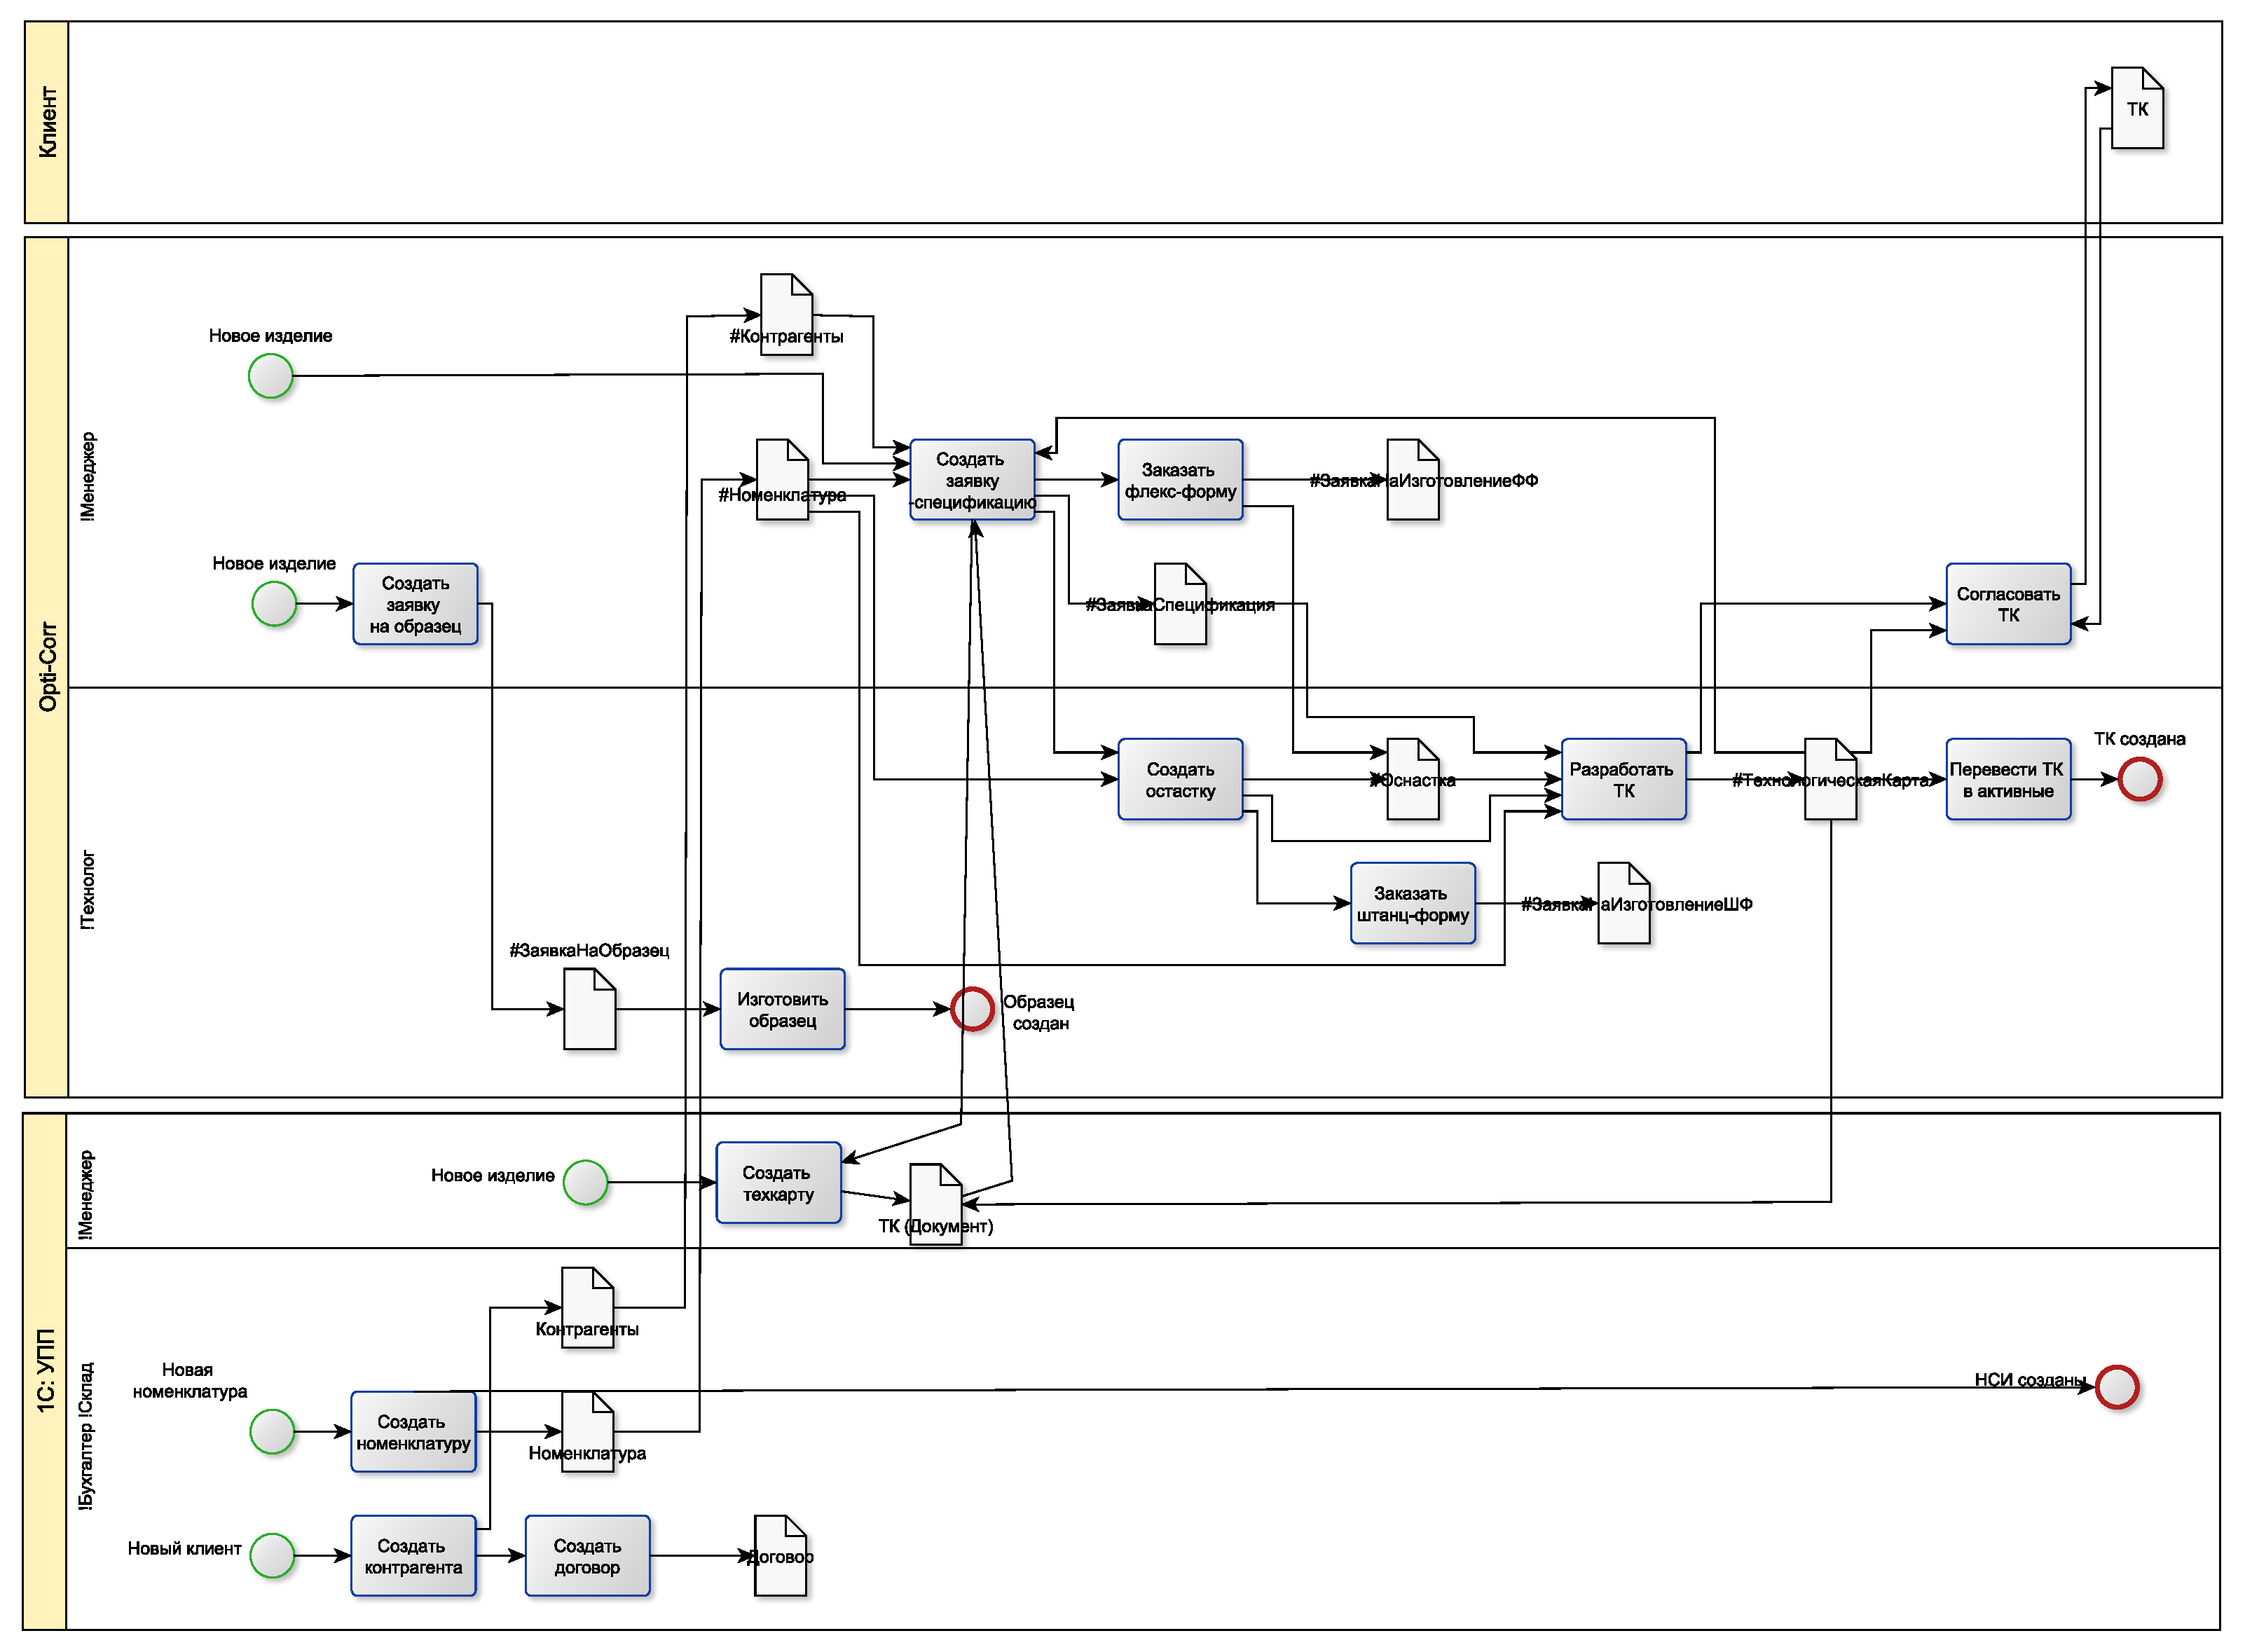
\includegraphics[width=200mm, height=220mm, angle=90, keepaspectratio]{50_Pics/1_NewGoods.pdf}
\caption{Схема бизнес-процесса ''Проектирование и разработка новой продукции''}
\label{pic:1_Newgoods}
\end{figure*} 

\clearpage



\begin{figure*}[!htb]
\centering
  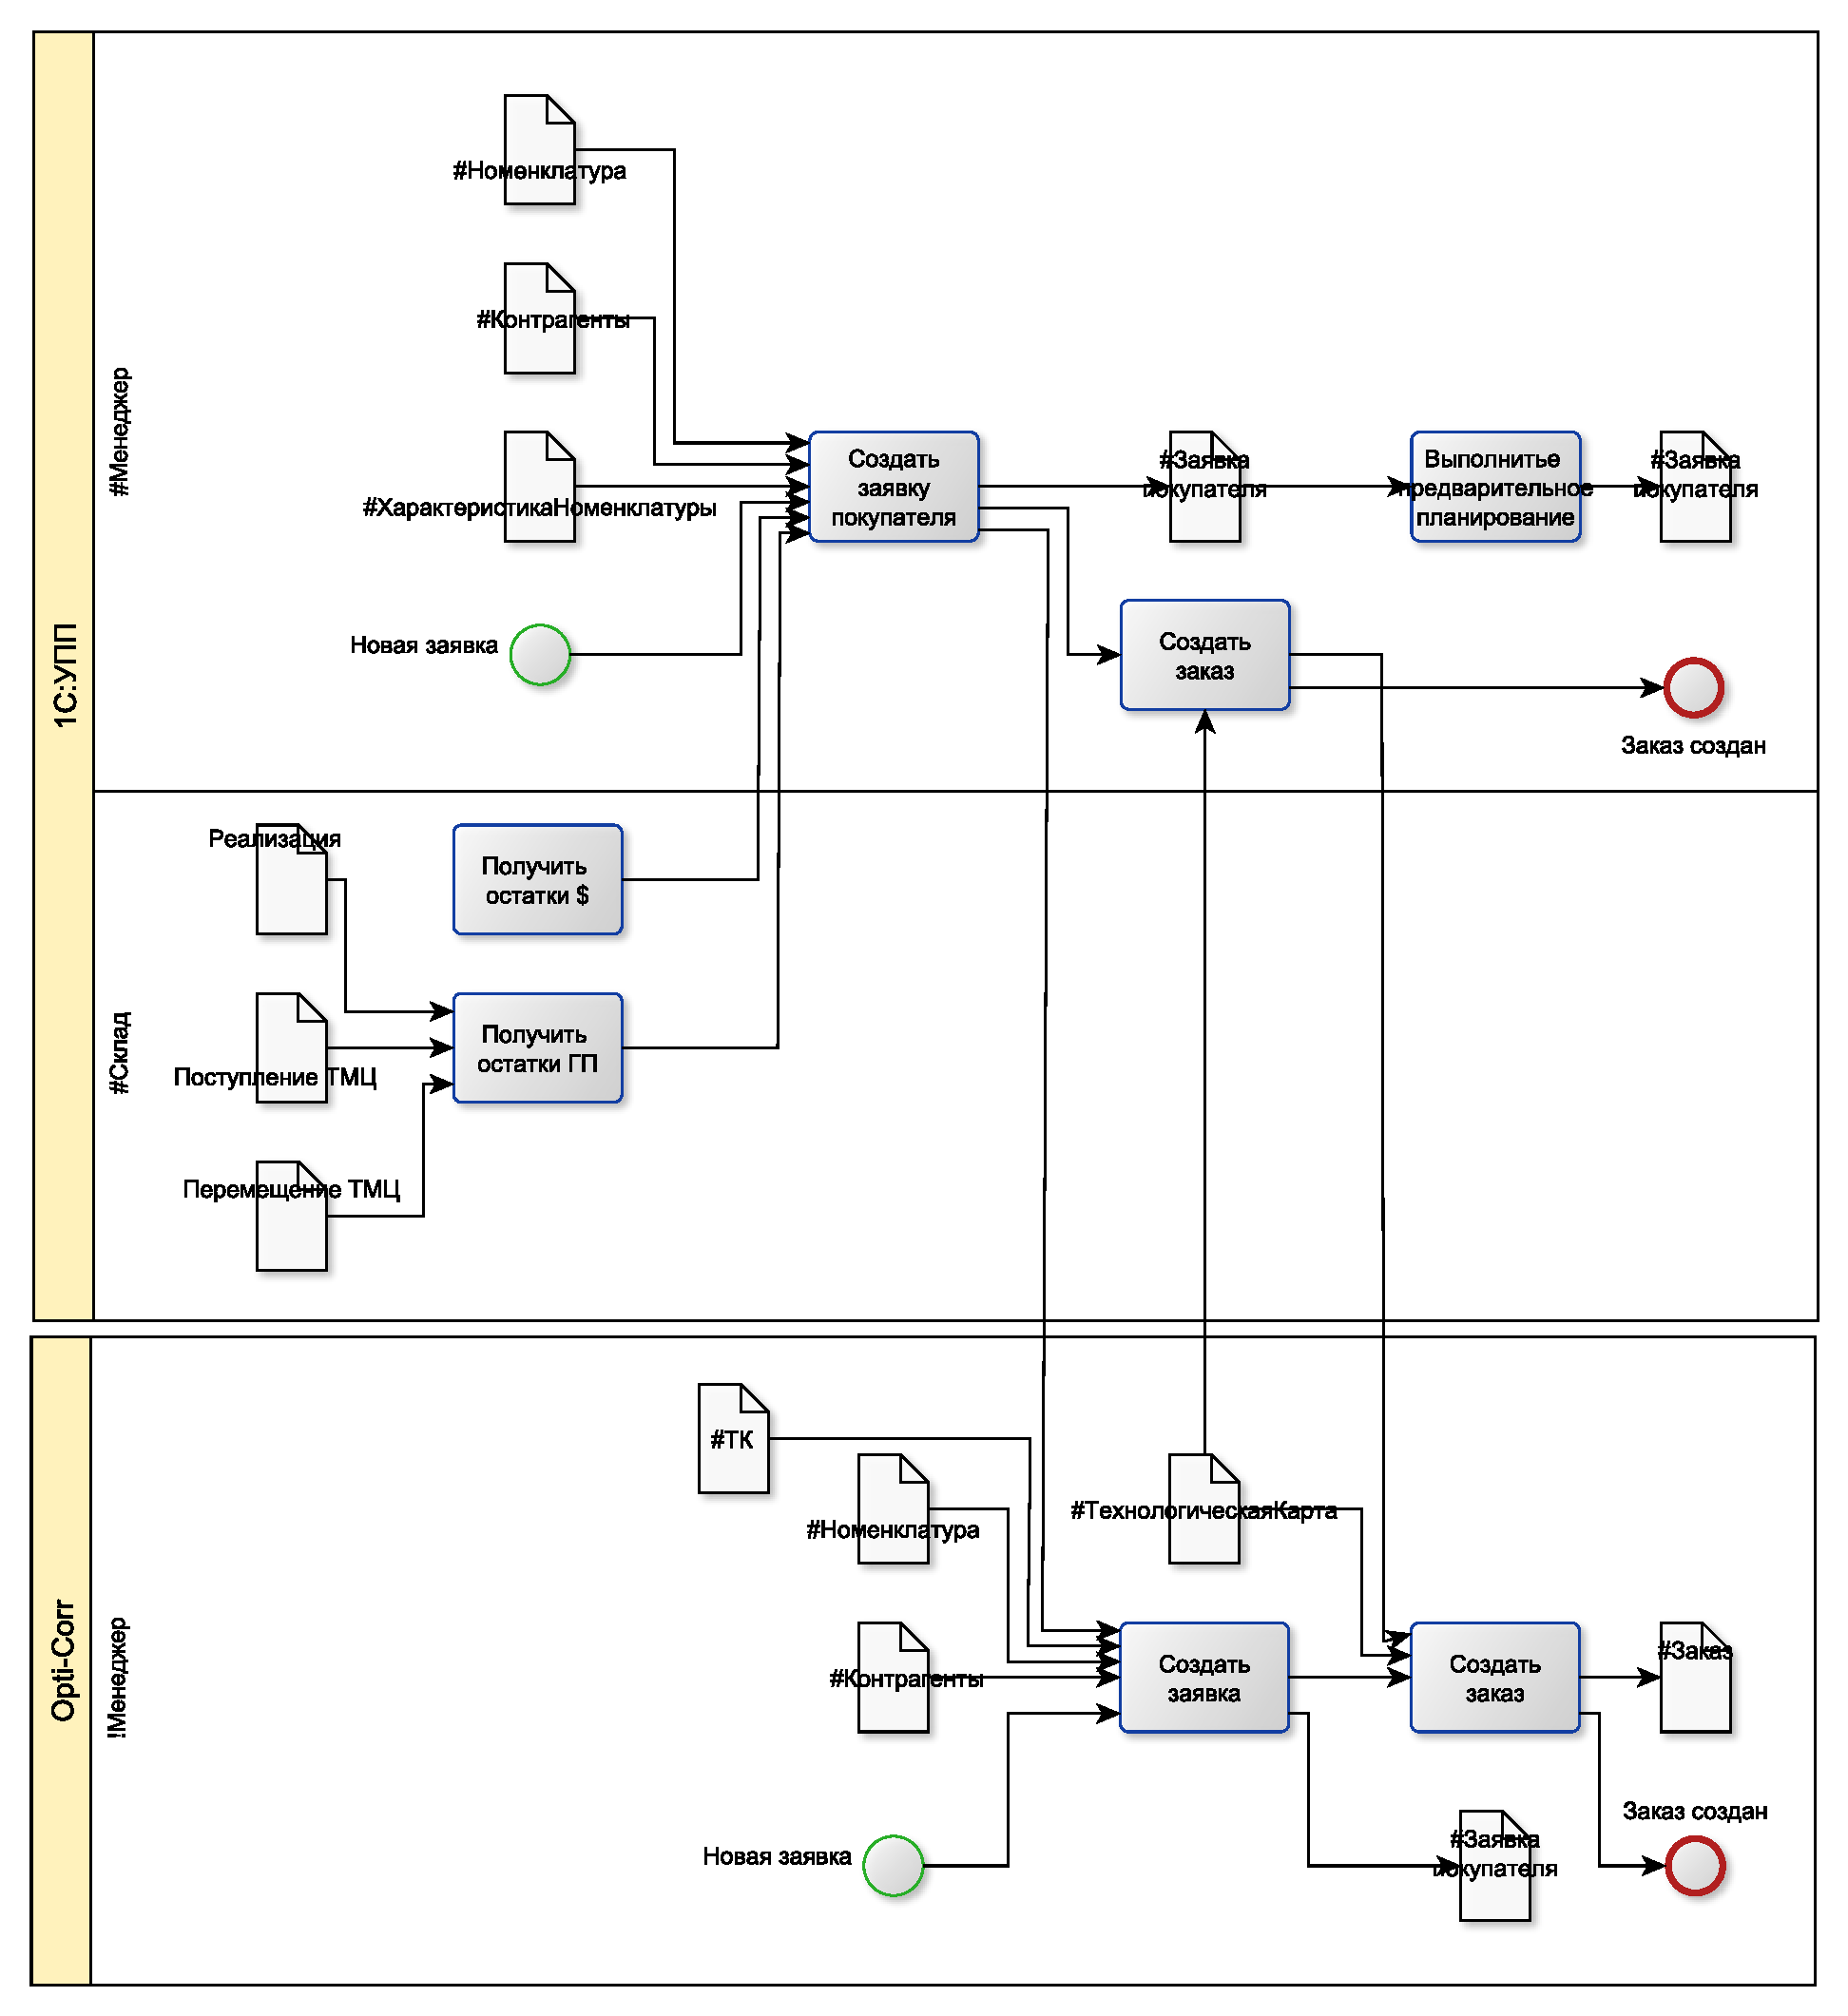
\includegraphics[width=180mm, height=180mm, angle=90, keepaspectratio]{50_Pics/2_Sales.pdf}
\caption{Схема бизнес-процесса ''Продажа готовой продукции''}
\label{pic:2_Sales}
\end{figure*} 

\clearpage


\begin{figure*}[!htb]
\centering
  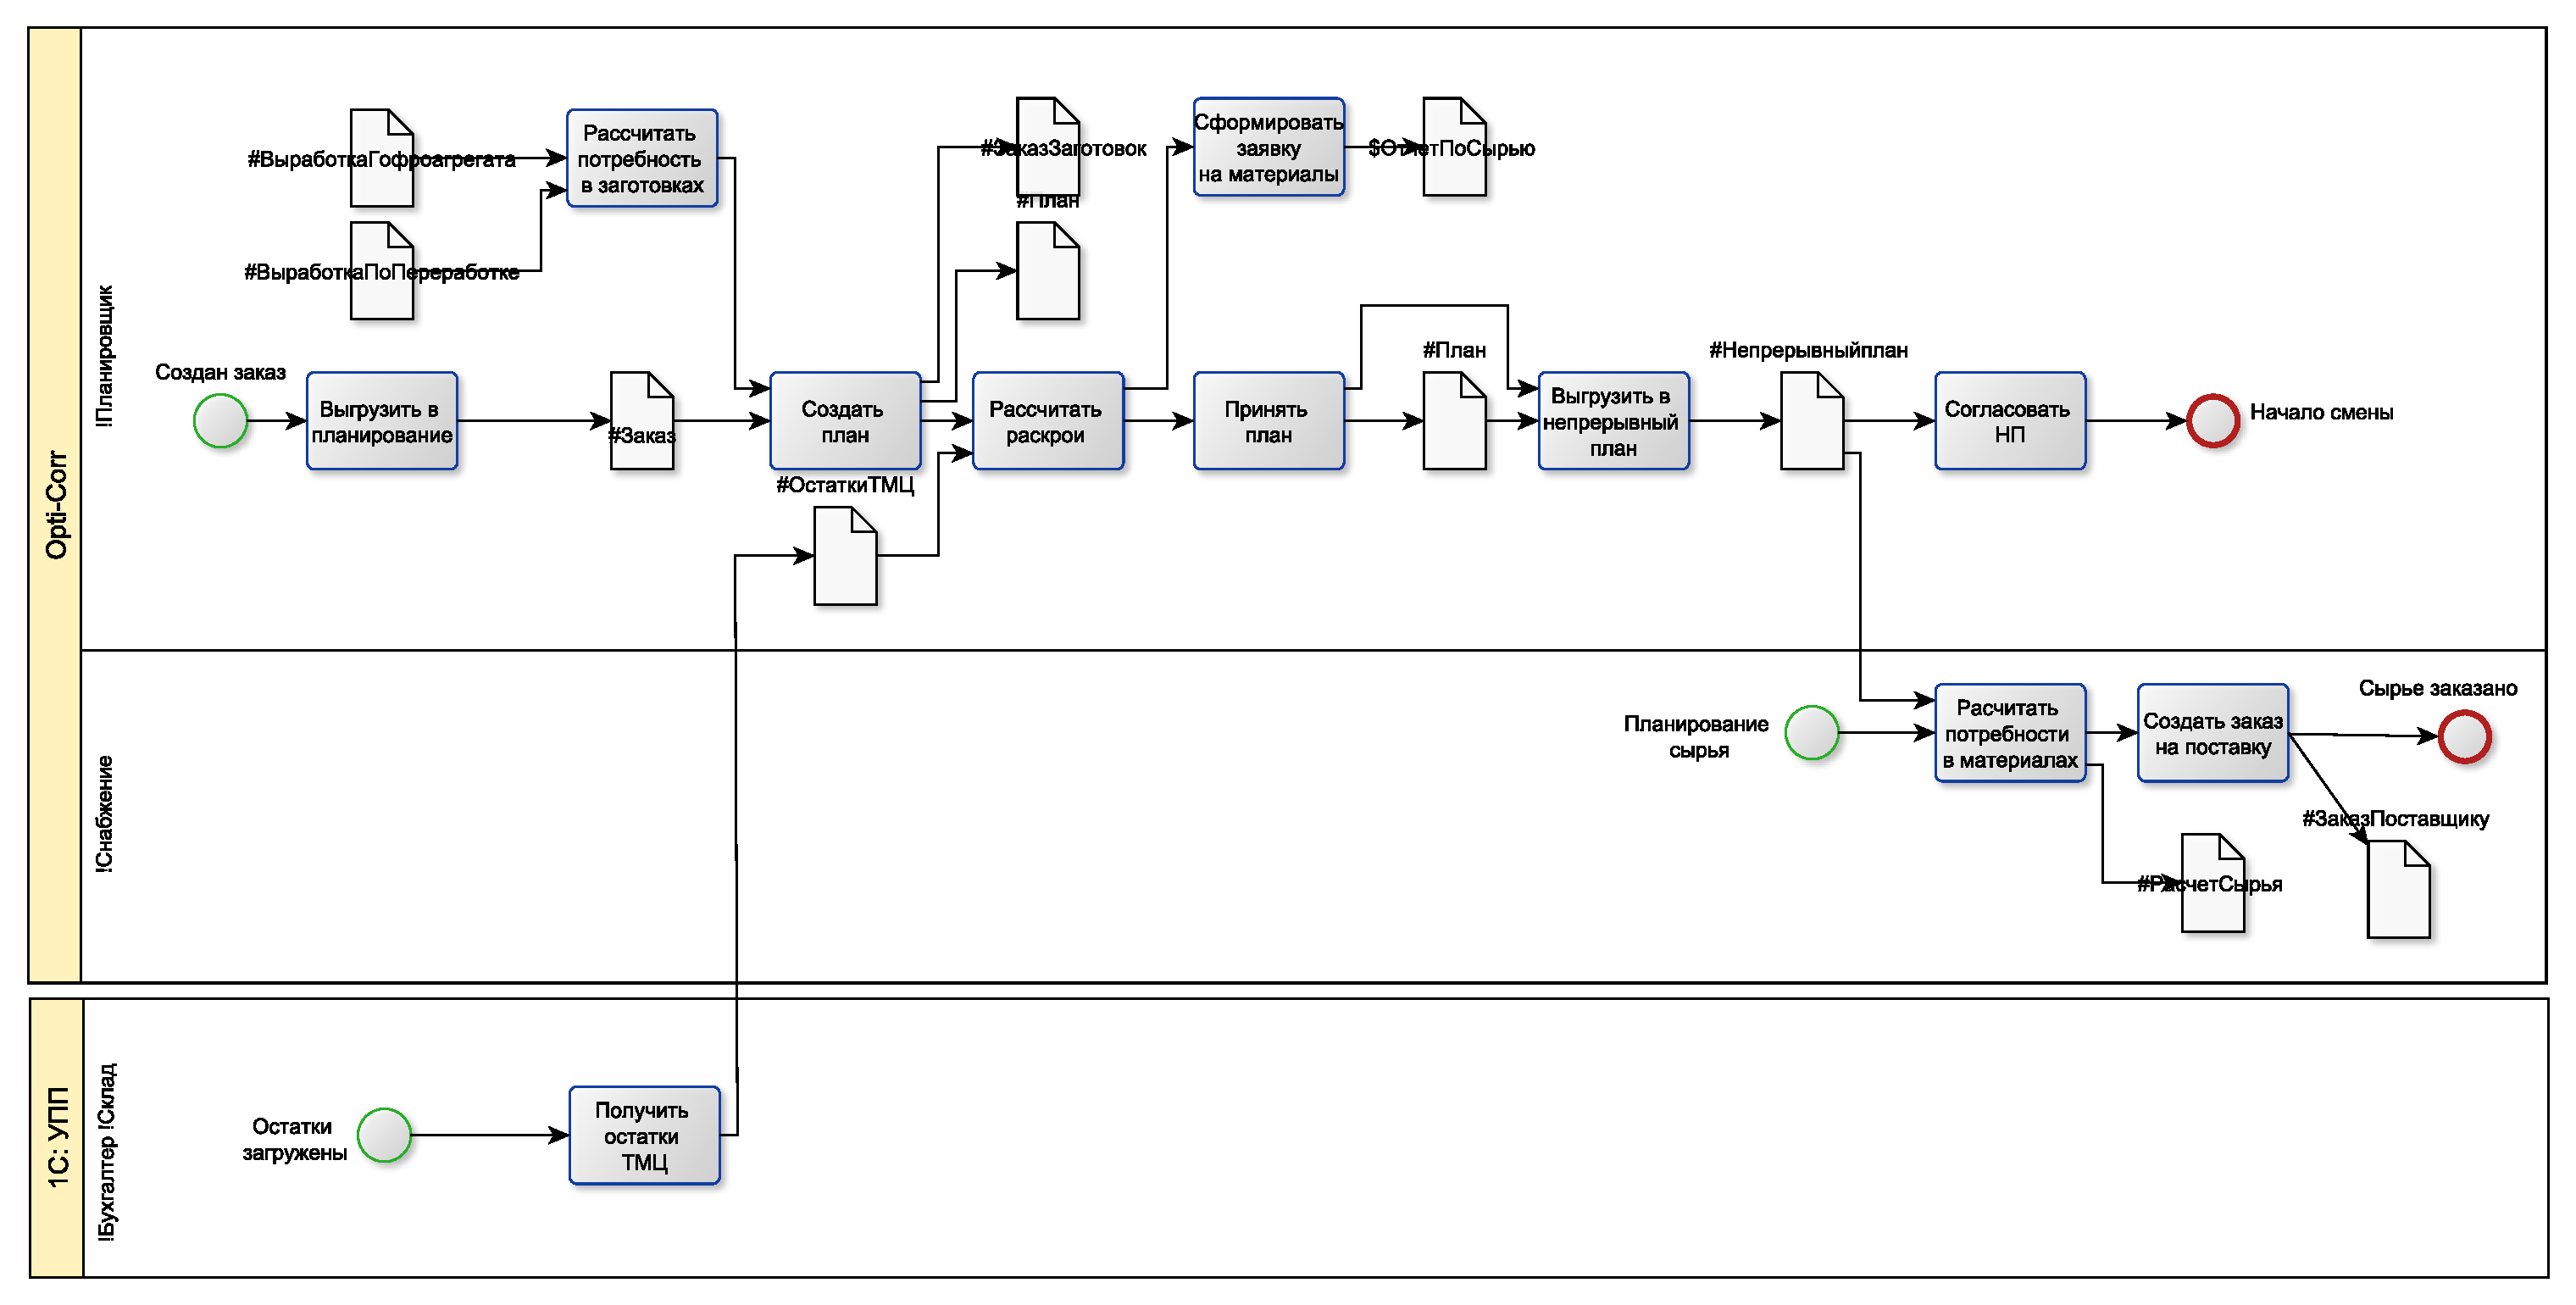
\includegraphics[width=200mm, height=220mm, angle=90, keepaspectratio]{50_Pics/3_Plan.pdf}
\caption{Схема бизнес-процесса ''Планирование производства''}
\label{pic:3_Planning}
\end{figure*} 

\clearpage


\begin{figure*}[!htb]
\centering
  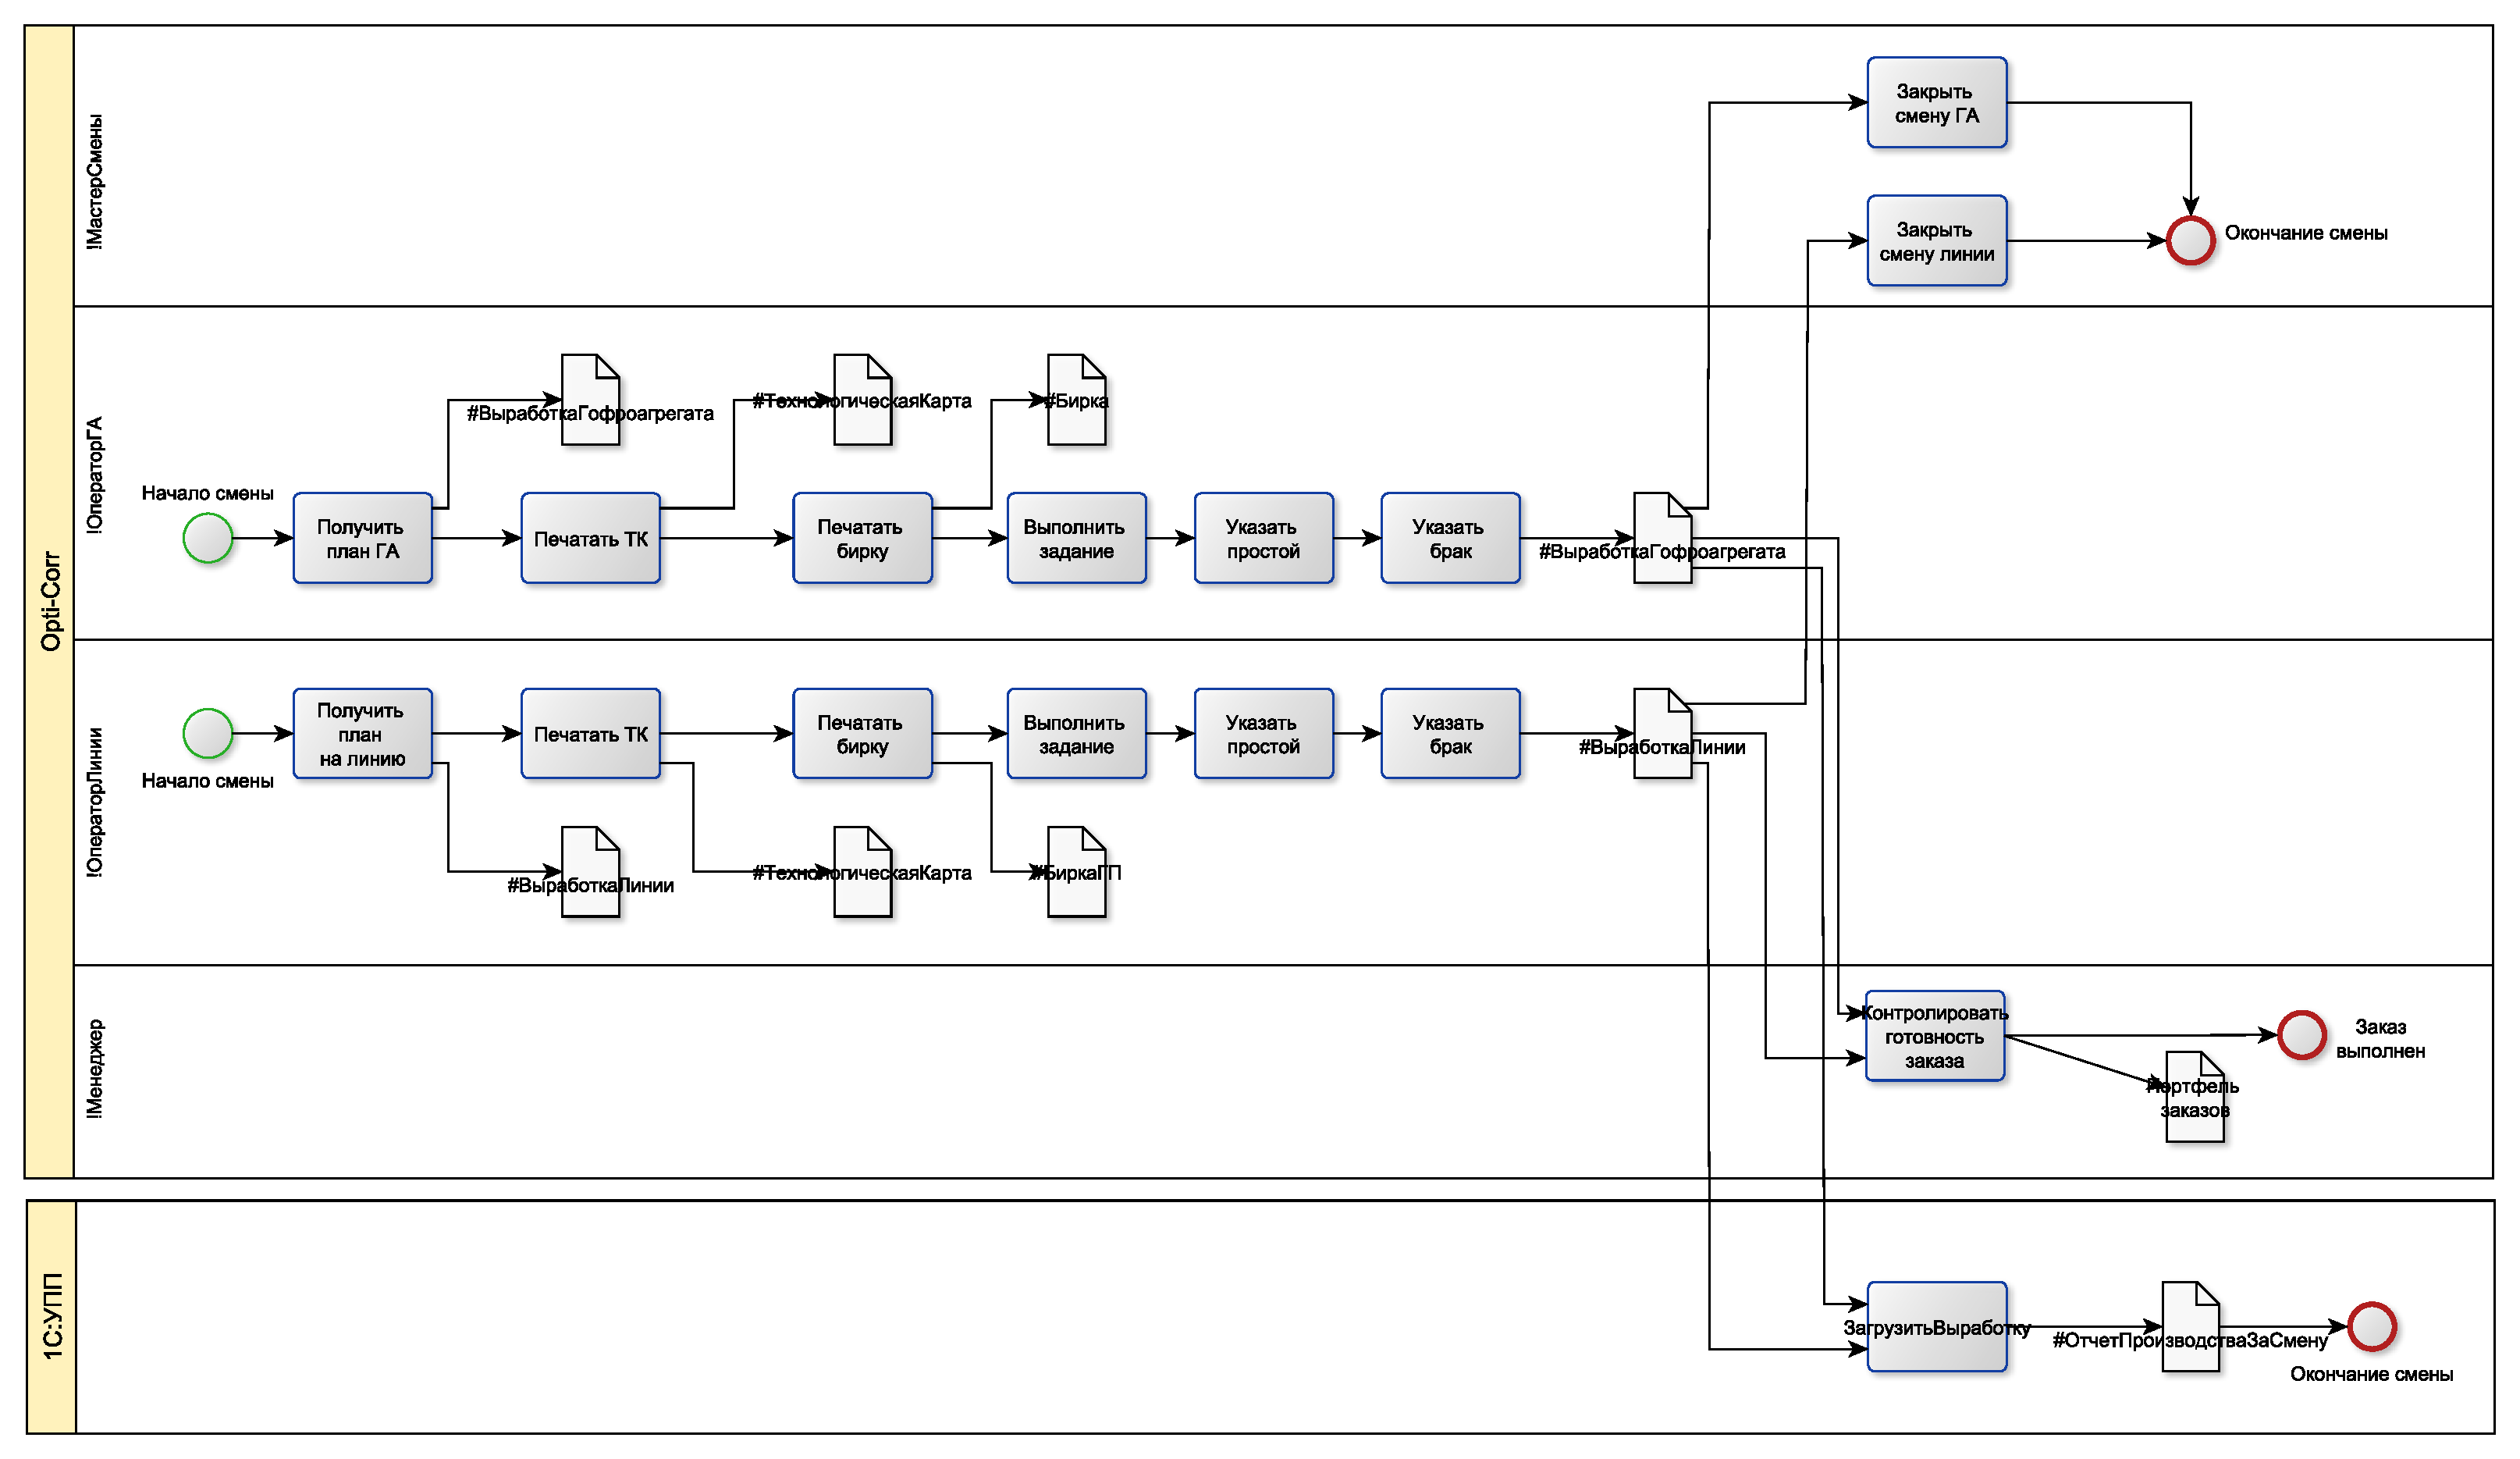
\includegraphics[width=200mm, height=220mm, angle=90, keepaspectratio]{50_Pics/4_Output.pdf}
\caption{Схема бизнес-процесса ''Выпуск готовой продукции и полуфабрикатов''}
\label{pic:4_Output}
\end{figure*} 


\begin{figure*}[!htb]
\centering
  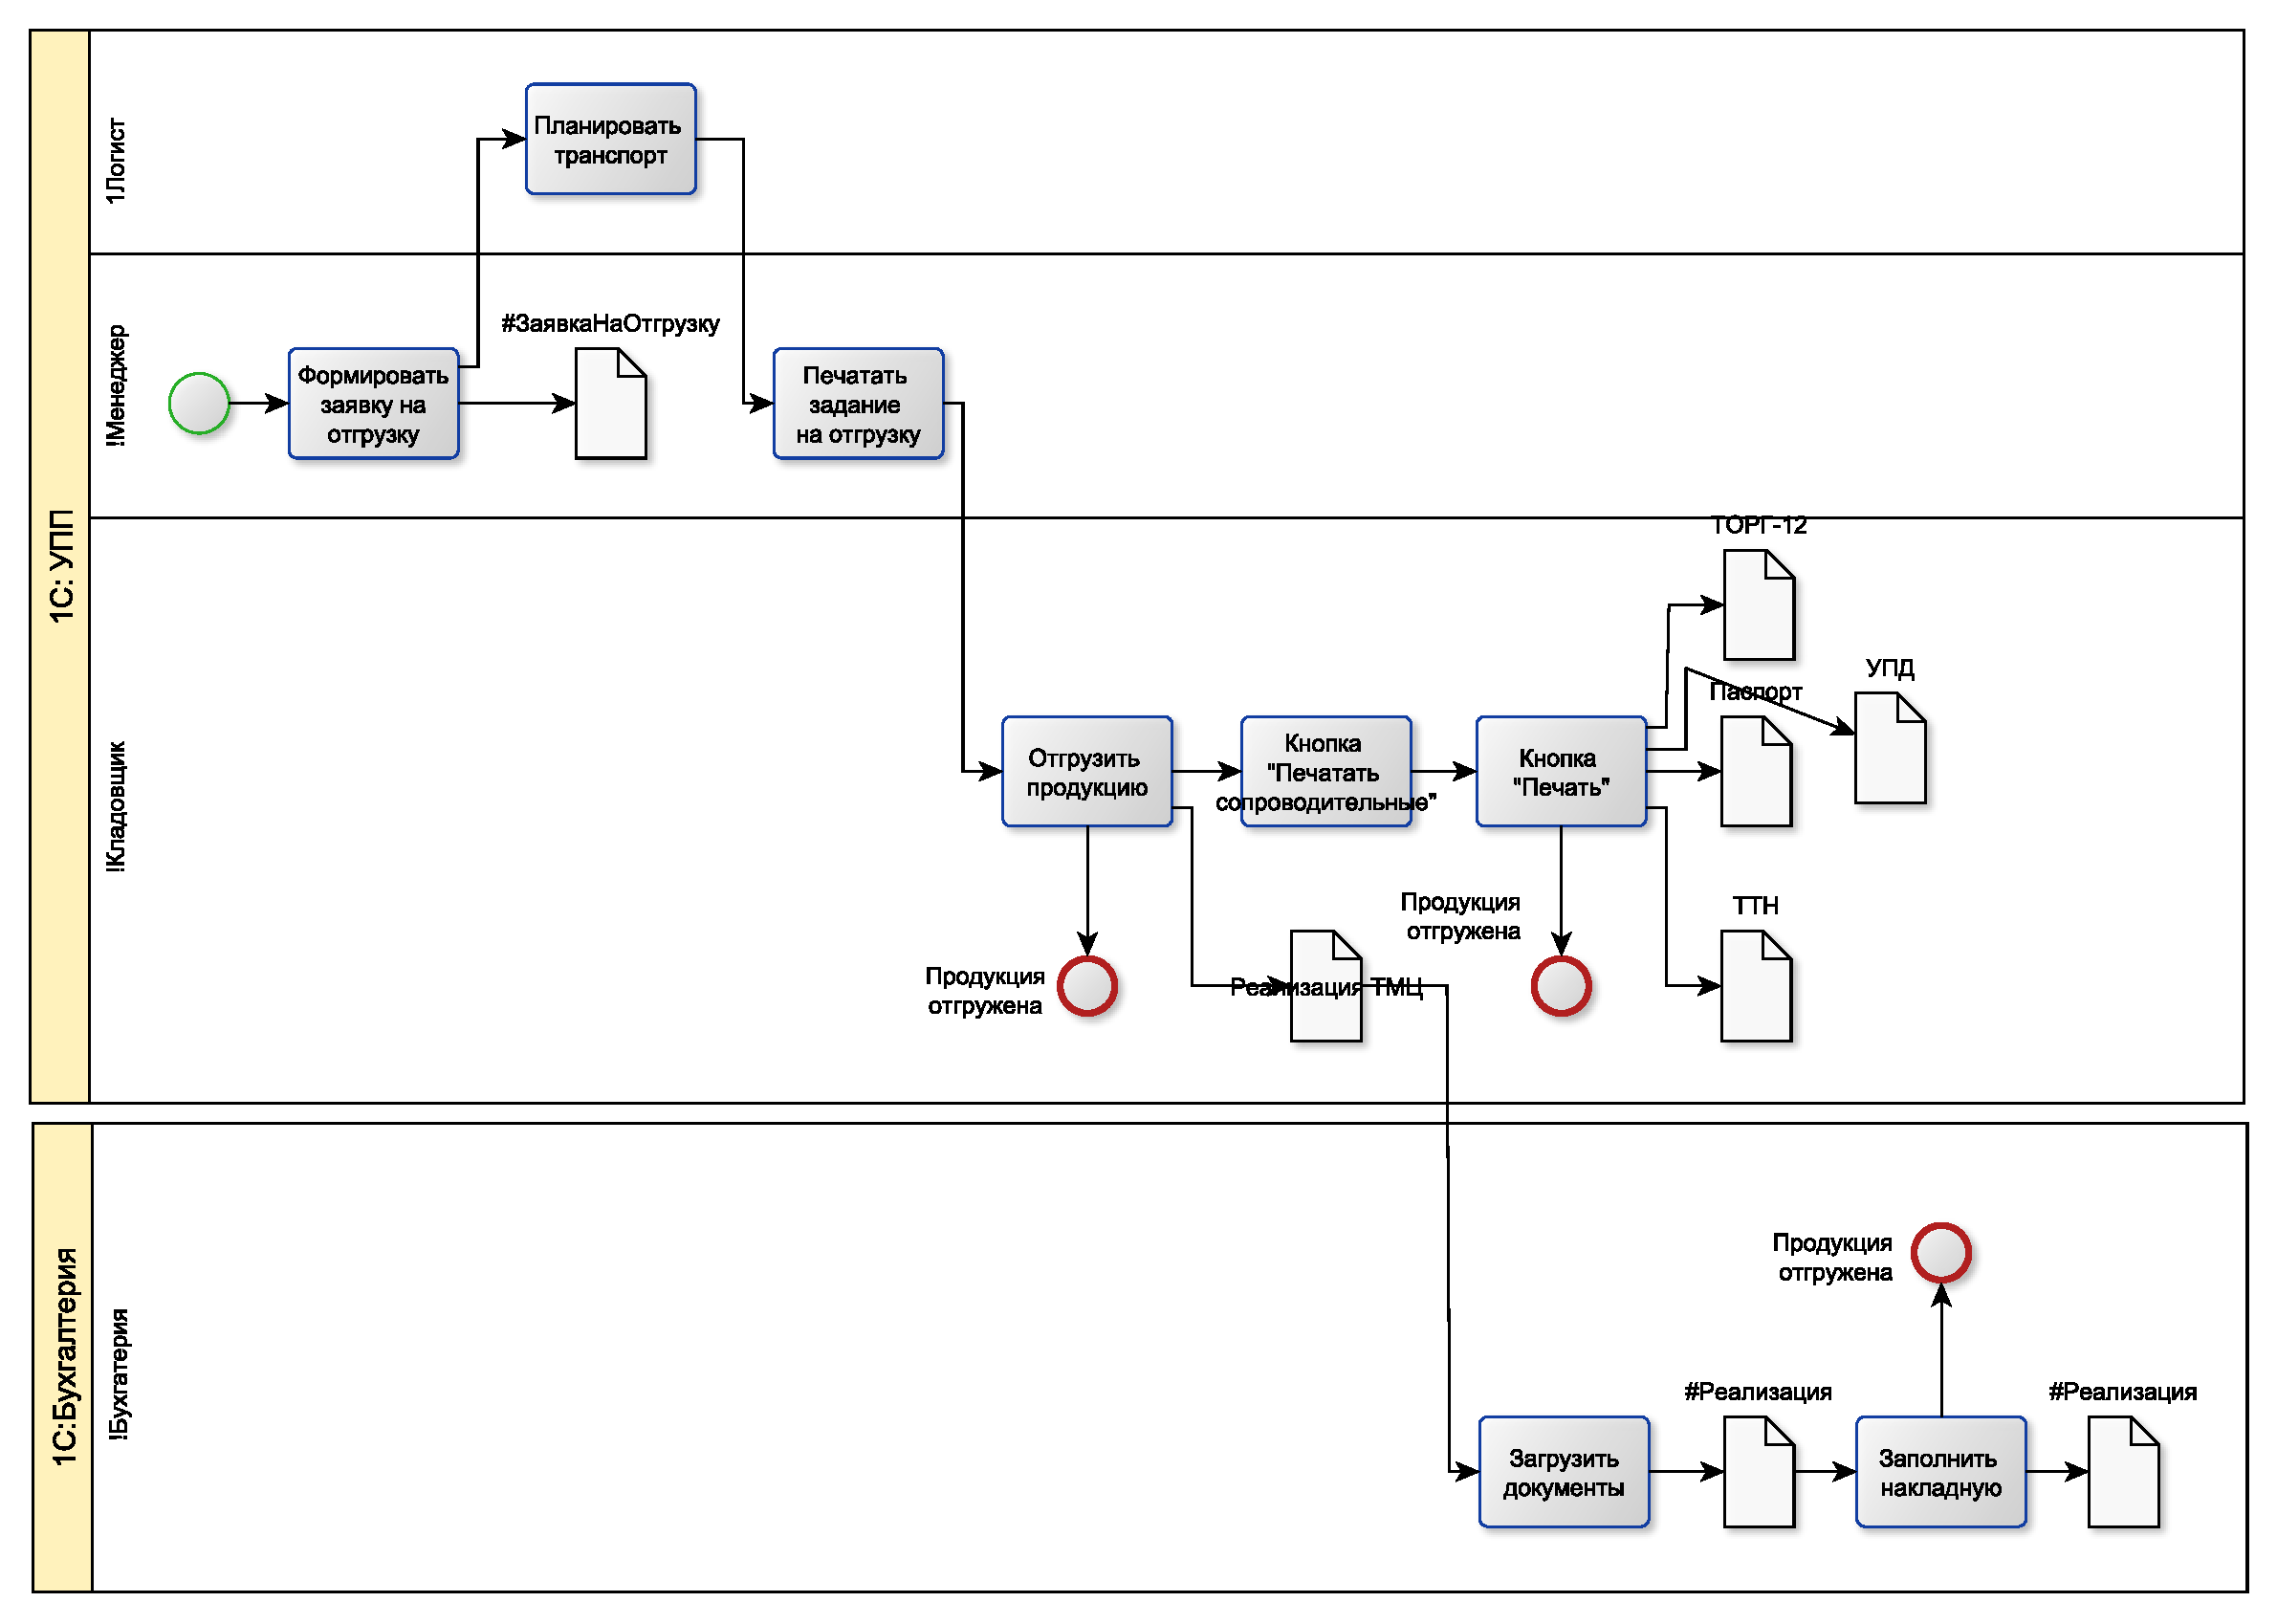
\includegraphics[width=200mm, height=220mm, angle=90, keepaspectratio]{50_Pics/5_Shipment.pdf}
\caption{Схема бизнес-процесса ''Отгрузка готовой продукции''}
\label{pic:4_Shipment}
\end{figure*} 

% \begin{figure*}[!htb]
% \centering
%   \includegraphics[width=200mm, height=220mm, angle=90, keepaspectratio]{50_Pics/6Warehouse.pdf}
% \caption{Схема бизнес-процесса ''Учет ТМЦ''}
% \label{pic:6_Stock}
% \end{figure*} 


\clearpage




\begin{comment} % ЗАККОМЕНТИРОВАН БЛОК 47-56

\begin{figure*}[!htb]
\centering
  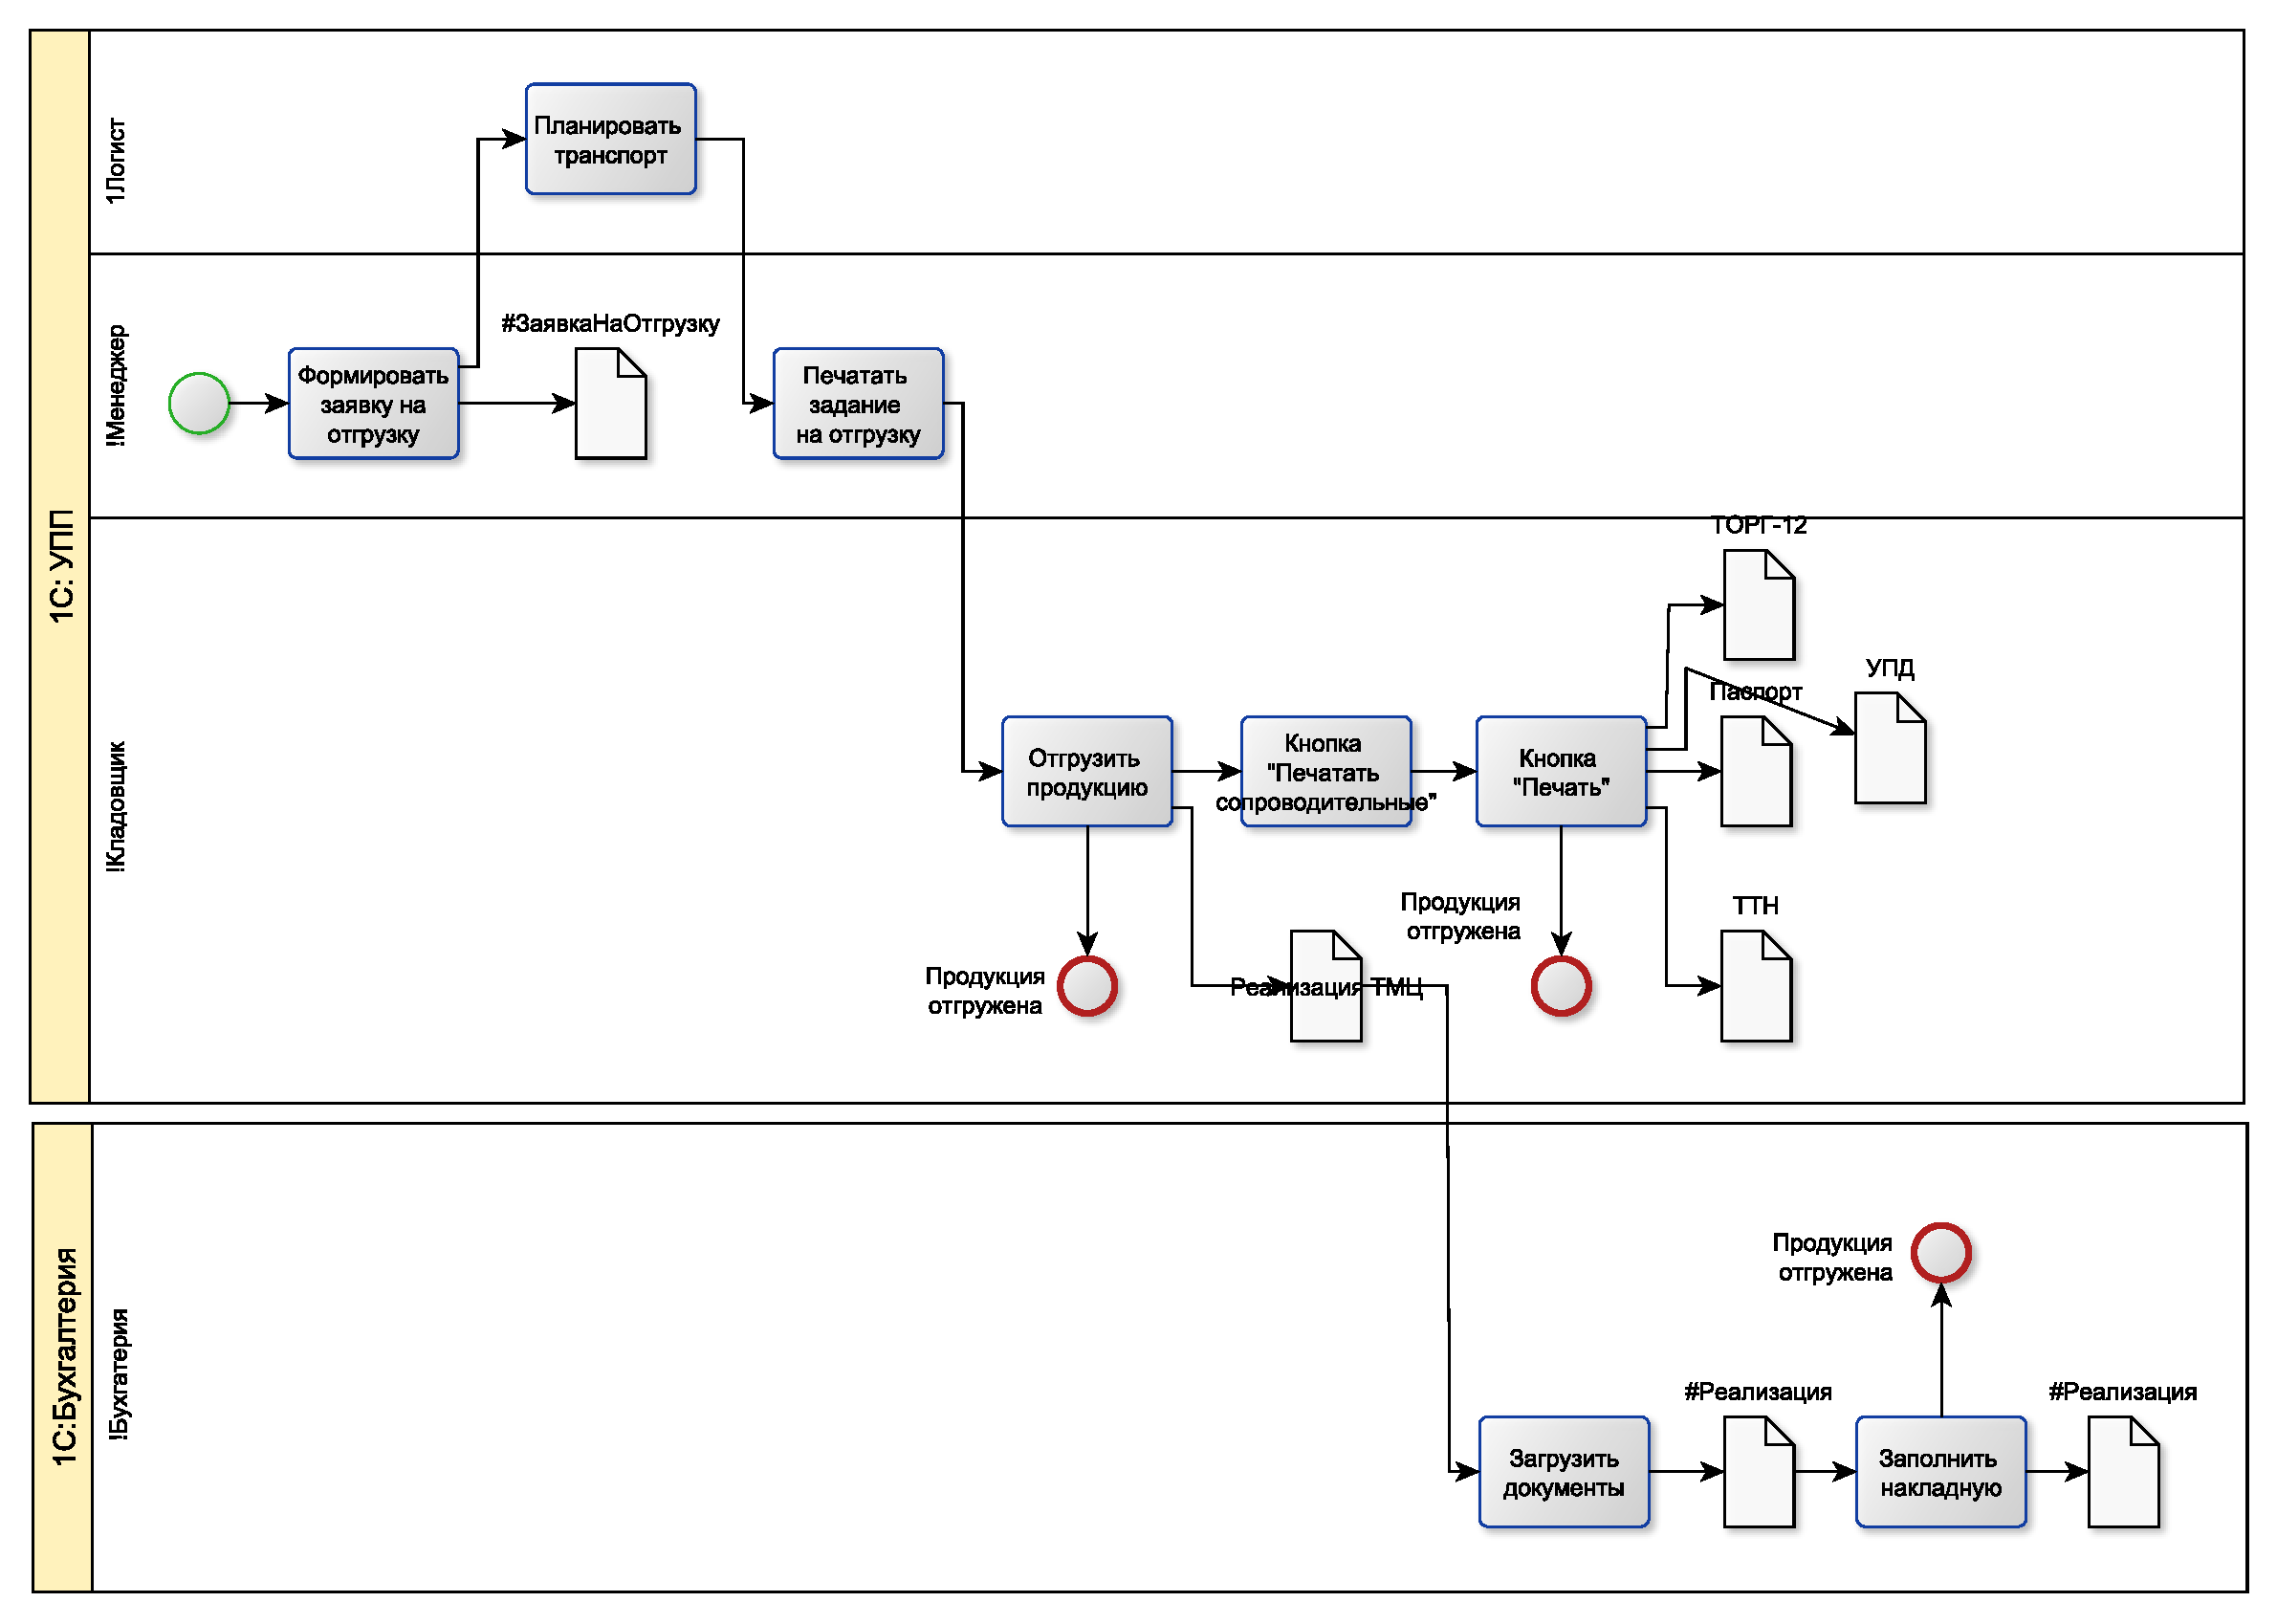
\includegraphics[width=200mm, height=220mm, angle=90, keepaspectratio]{50_Pics/5_Shipment.pdf}
\caption{Схема бизнес-процесса ''Отгрузка готовой продукции''}
\label{pic:bp_shipment}
\end{figure*} 

\end{comment}

\clearpage  % схемы
 	
 	% 
\newpage
\section{Приложение B. Карта рабочих мест}

\pc

\newcounter{workplace}
\setcounter{workplace}{0}

% Table generated by Excel2LaTeX from sheet 'Лист1'
\scriptsize
\begin{longtable}{|p{10mm}|p{50mm}|p{30mm}|p{40mm}|p{20mm}|}
\hline
{ {\bf \parbox[c][10mm]{10mm}{\centering №}}} & { {\bf \parbox[c]{50mm}{\centering Должность}}} & { {\bf \parbox[c]{30mm}{\centering Структурное подразделение}}} & { {\bf \parbox[c]{40mm}{\centering Роль}}} & { {\bf \parbox[c]{20mm}{\centering Количество}}} \\
\hline
\p & Дизайнер-конструктор & Отдел разработки ТК & \tehnolog & 1 \addtocounter{workplace}{1} \\
%\hline
%\p & Дизайнер & Отдел продаж & \designer & 1 \addtocounter{workplace}{1} \\
% \hline
% \p &  Дизайнер и конструктор & Дизайн-студия & \designer и \tehnolog & 1 \addtocounter{workplace}{1} \\


\hline
\p &  Планировщик  & Отдел планирования  & \planner & 1
\addtocounter{workplace}{1} \\
\hline
\p &   Директор по производству & Производственный отдел & { {\parbox{50mm}{\processengineer}}} & 1 \addtocounter{workplace}{1} \\
\hline
\p &  Мастер смены & Производство & \master & 1 \addtocounter{workplace}{1} \\
\hline
\p & Бригадир  гофроагрегата & Производство & \gaoperator & 1 \addtocounter{workplace}{1} \\

\hline
\p &  Оператор линии & Производство & \operator & 
6 \addtocounter{workplace}{9} \\
%\hline
%\p &  Машинист  гофроагрегата. Мокрая часть  & Производство& \linkoperator & 1 \addtocounter{workplace}{1} \\


%\hline
%\p & Менеджер отдела маркетинга и продаж & Отдел маркетинга и продаж & \manager & 3 \addtocounter{workplace}{6} \\
\hline
\p &  Менеджер по продажам & { \parbox{38mm}{Отдел продаж }} & {\parbox{50mm}{\manager}} & 3 \addtocounter{workplace}{3} \\
%\hline
%\p &  Слесарь-монтажник & Планово-производственный отдел  & \montaznik & 2 \addtocounter{workplace}{2} \\
% \hline
% { \parbox[c][10mm]{16mm}{11}} &  Комплектовщик & { \parbox{38mm}{Отдел подготовки производства}} & { {\bf \parbox{50mm}{!Комплектовщик}}} & 
% 1 \addtocounter{workplace}{1} \\
%\hline
%\p &  Инженер планово-производственного отдела & Планово-производственный отдел &  \planner & 1 \addtocounter{workplace}{1} \\

%\hline
%\p &  Инженер-технолог производства & Планово-производственный отдел &  \prodtehnolog & 1 \addtocounter{workplace}{1} \\

% \hline
% \p &  Технолог производства & Планово-производственный отдел &  \prodtehnolog & 1 \addtocounter{workplace}{1} \\

\hline
\p & Кладовщик & Складское хозяйство &  \kladovshik & 1 \addtocounter{workplace}{1} \\

\hline
\p & Экономист & Финансовый отдел & { {\parbox{50mm}{\auditor}}} &  1 \addtocounter{workplace}{1} \\

\hline
\p & Директор & Администратор & \director &  1 \addtocounter{workplace}{1} \\
\hline
& & & ИТОГО & \theworkplace \\
\hline
\caption{Карта рабочих мест}\label{tab:usercount}
\end{longtable}  
\normalsize

  % карта рабочих мест 
\end{document}
